\chapter{SOI刻蚀中的显色特性研究}
\section{背景介绍}

在SOI平台器件加工的过程中,标准SOI的硅层厚度通常只有几个固定的值,比如220~$nm$,340~$nm$,如图\ref{color_wafer}所示。图\ref{color_wafer}(a)所示为硅层厚度220~$nm$的12英寸SOI芯片,其颜色显示为淡绿色,但由于硅层厚度的不均匀性,中间与边缘区域表现为淡紫色。图\ref{color_wafer}(b)所示为硅层厚度340~$nm$的12英寸SOI芯片,其颜色显示为淡紫色,但由于硅层厚度的不均匀性,边缘区域表现为淡绿色。上述颜色均为日光灯下接近垂直视角所拍摄的颜色。

\begin{figure}[htb]
	\centering
	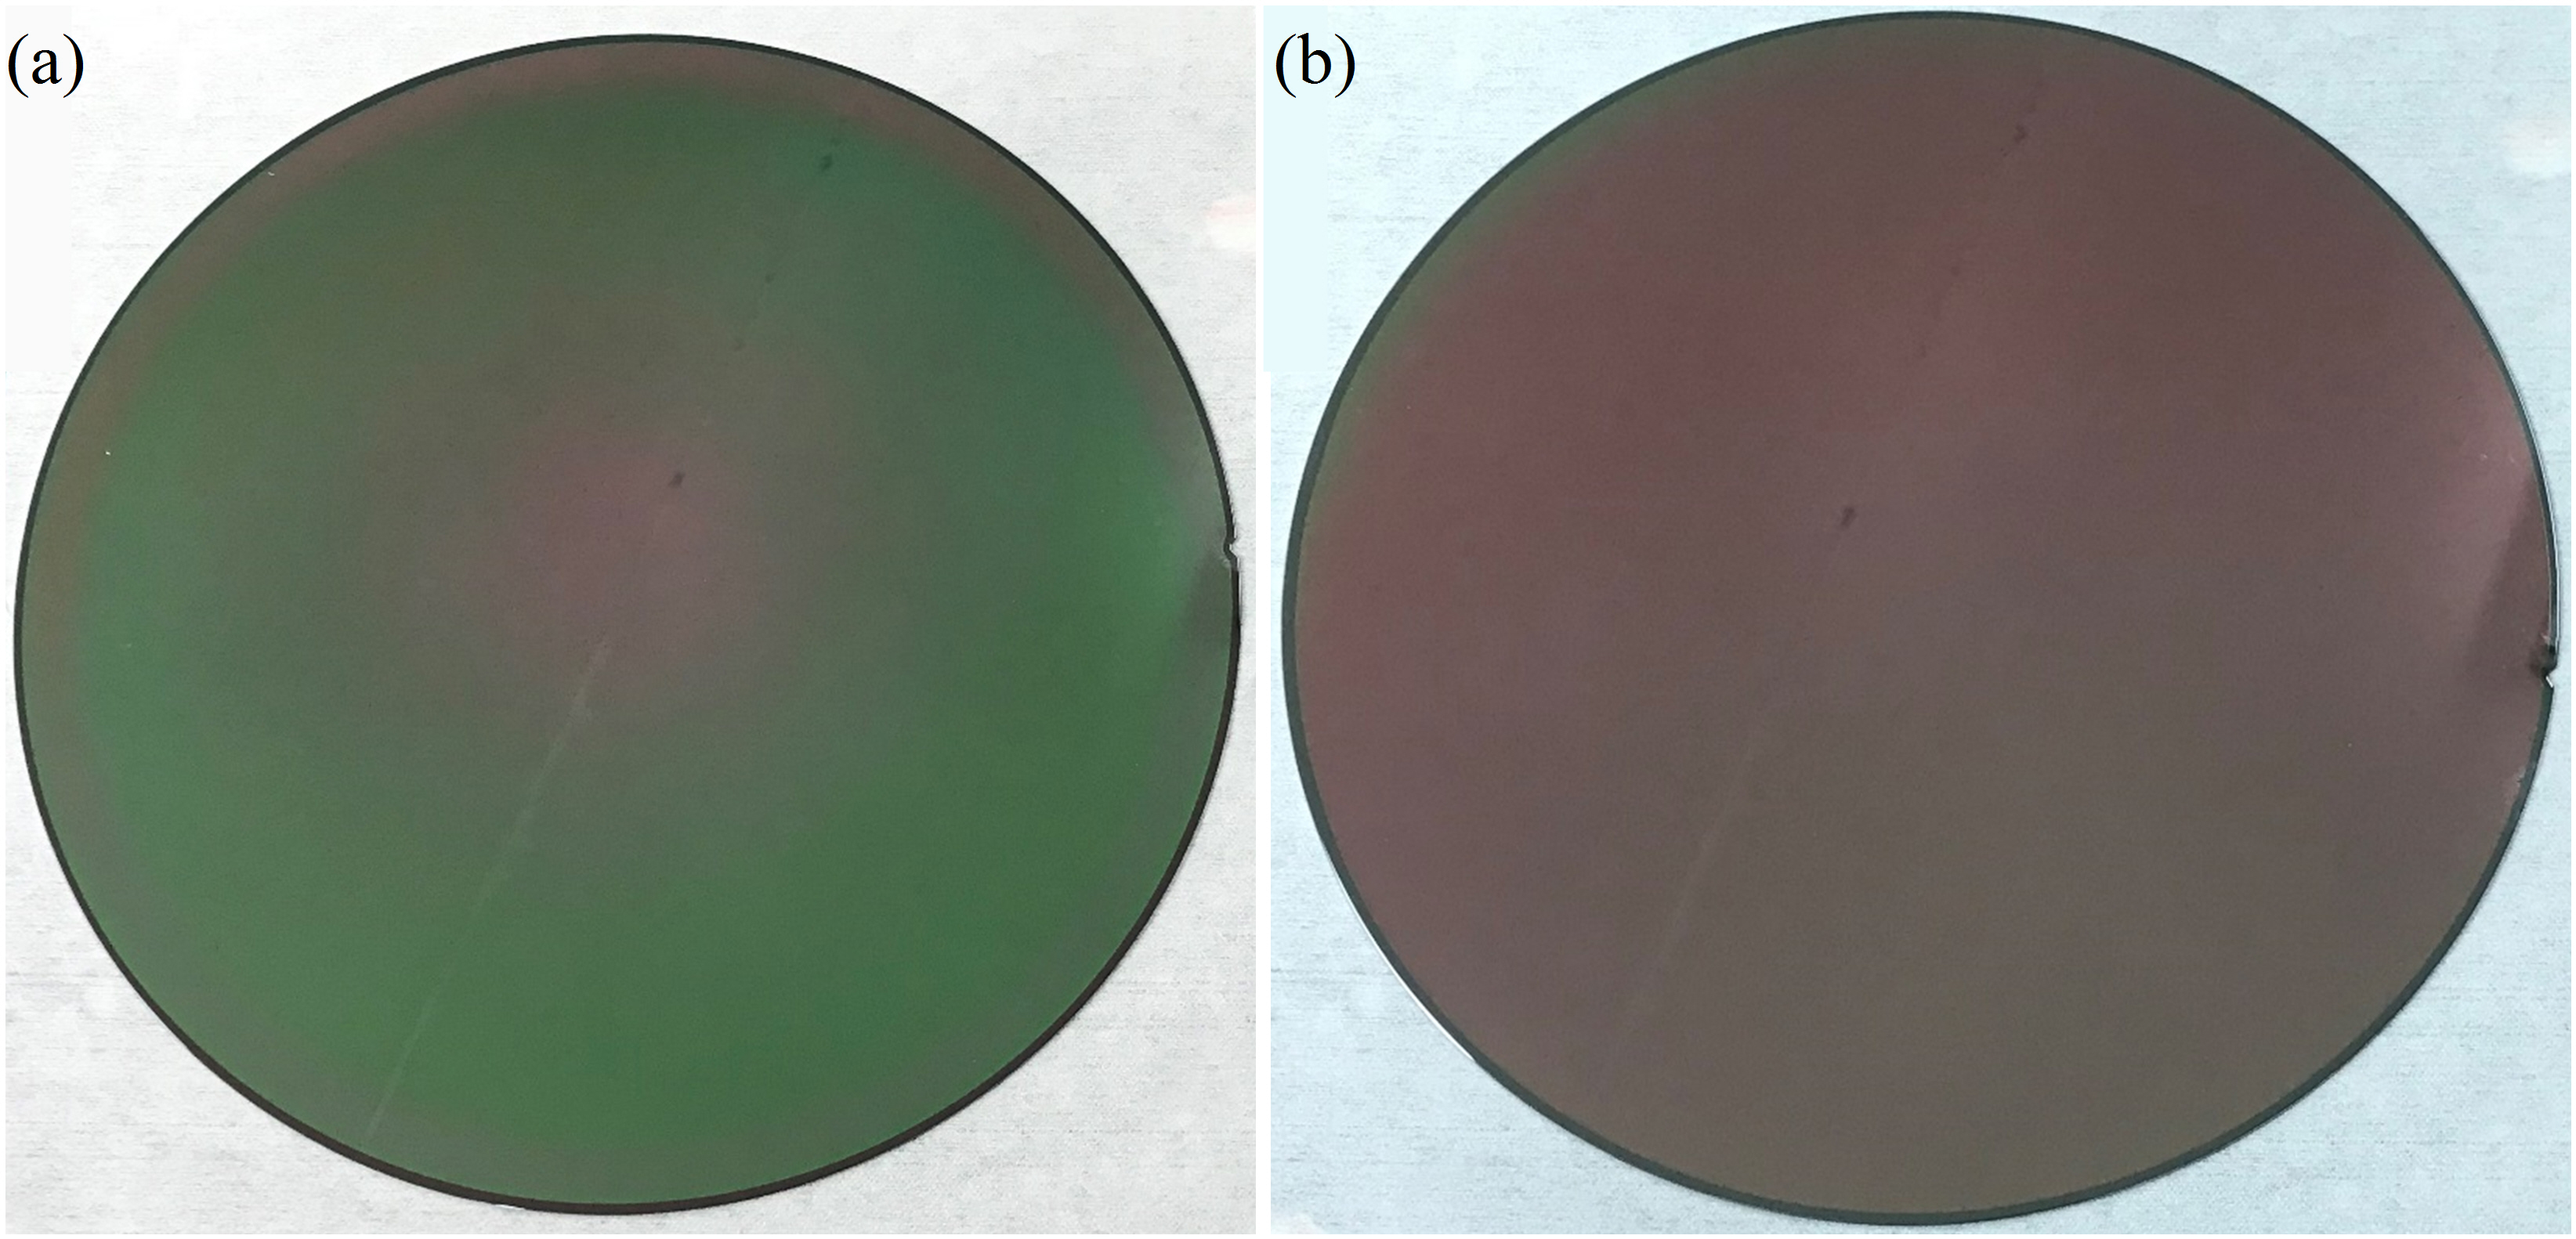
\includegraphics[width=14cm]{./Pictures/color_wafer.jpg}
	\captionsetup{justification=centering}
	\caption{标准12英寸SOI芯片,(a)~220~$nm$硅层厚度;(b)~340~$nm$硅层厚度}
	\label{color_wafer}
\end{figure}

传统的硅波导的厚度大约在200~\~{}500~$nm$之间,近年来人们开始研究超薄硅波导,其相较于220~$nm$厚的传统硅波导来说,有以下几种优势:首先,因为超薄硅波导中的模式相对于传统波导中的模式对侧壁粗糙度更加不敏感,所以其传输损耗相比于传统220~$nm$厚的硅波导来说可以降低,Dumon等人测得对于高度为220~$nm$的硅波导,当波导宽度分别为400~$nm$、450~$nm$和500~$nm$时,其在1550~$nm$对应的损耗分别为33.8~dB/$cm$、7.4~dB/$cm$和2.4~dB/$cm$\cite{dumon2004low},Zou等人制作的高度为60~$nm$,宽度为950~$nm$的硅波导,损耗降到了0.61~dB/$cm$\cite{zou201560}。其次,由于超薄硅波导对光的限制能力变弱,等效折射率会降低,使得器件特征尺寸可以相对增大,更容易用较低成本的光刻技术加工\cite{zou201560}。超薄硅波导满足单模条件的波导宽度的也会更宽,且当波导宽度越大的时候,等效折射率对波导宽度的变化率就会降低,故超薄硅波导的制作容差就会变大。还有,对于模式转换器件来说,超薄硅波导的模式限制较弱,这意味着模式之间的重叠会增多,更容易实现超短的转换结构。在传感领域,由于超薄硅波导的模式限制较弱,故可以增强光场与物质的相互作用,从而提高器件的灵敏度。最后,由于超薄硅波导的宽高比很大,故可以减轻刻蚀过程中的迟滞效应\cite{jansen1997bsm},更容易制作波导之间的缝隙,并且该缝隙也更容易用二氧化硅等包层材料进行填充。

\begin{figure}[htb]
	\centering
	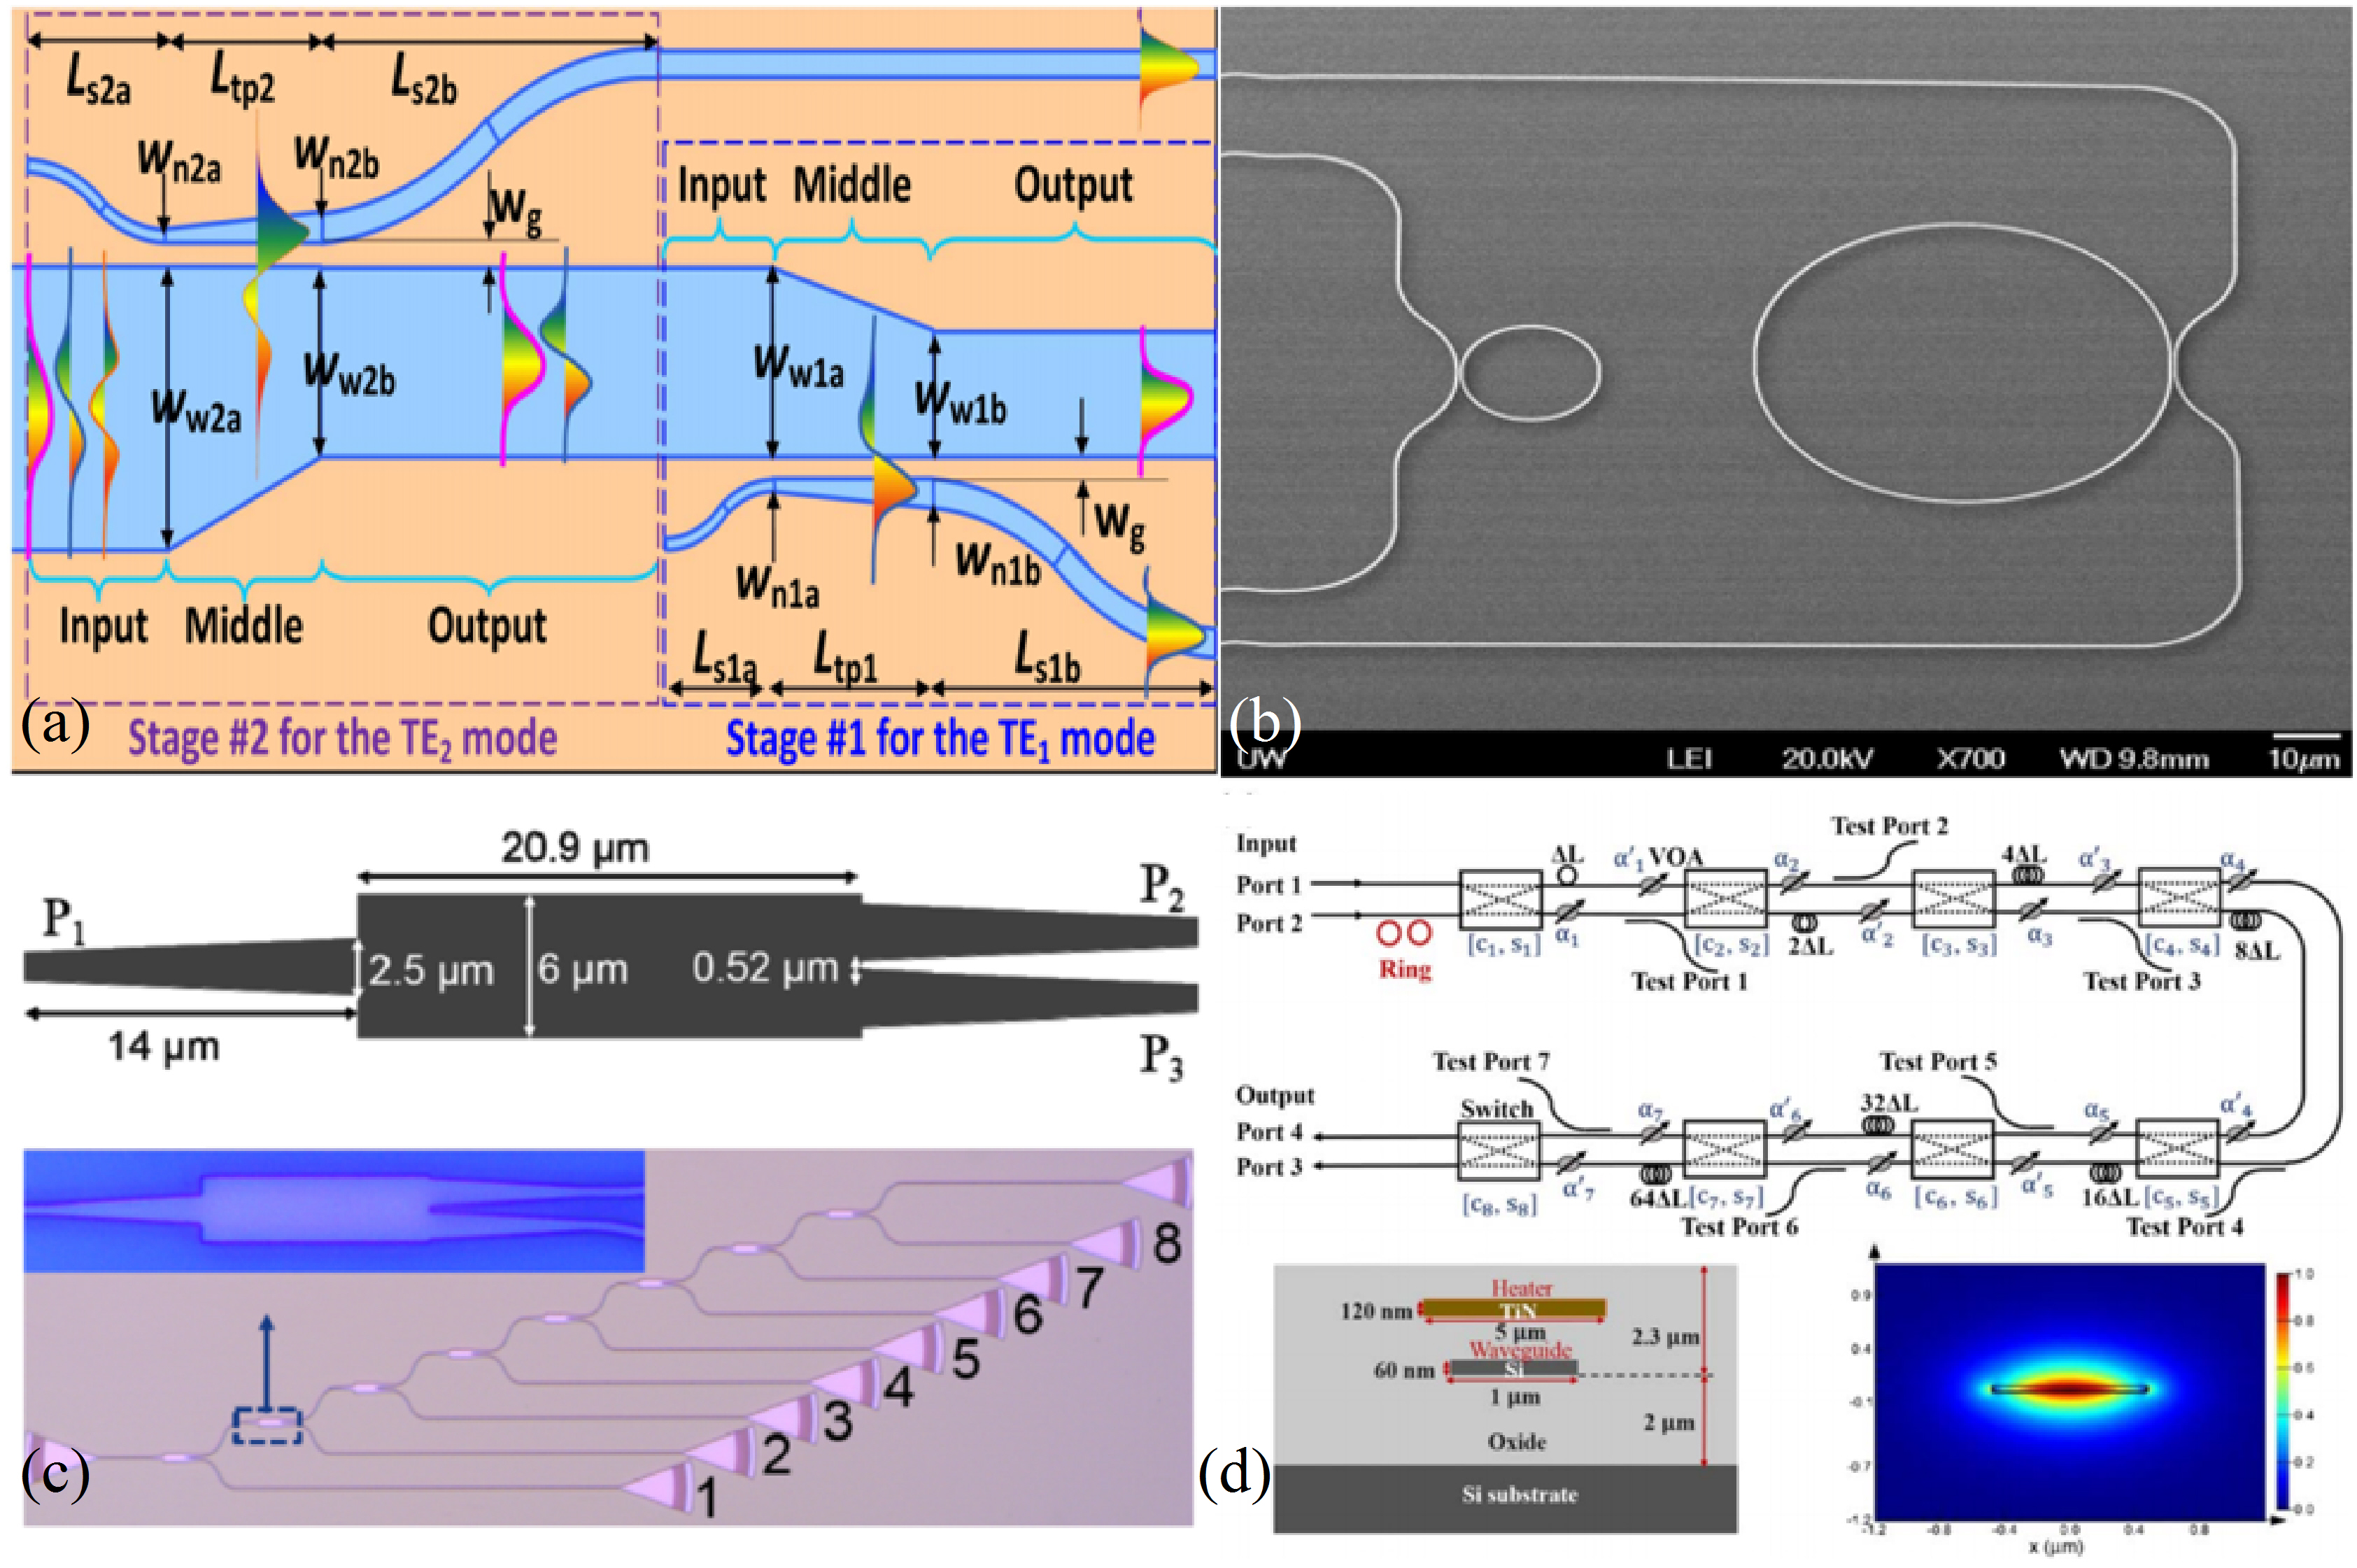
\includegraphics[width=14cm]{./Pictures/color_thin_application.jpg}
	\captionsetup{justification=centering}
	\caption{超薄硅器件,(a)模分复用解复用器,硅层厚度为50~$nm$\cite{li2017low};(b)微环传感器,硅层厚度为90~$nm$\cite{fard2014performance};(c)多模干涉耦合器,硅层厚度为60~$nm$\cite{zou201560};(d)延时线,硅层厚度为60~$nm$\cite{wang2017continuously}}
	\label{color_thin_application}
\end{figure}

利用超薄硅波导,Li等人制作了一个模分复用解复用器\cite{li2017low},如图\ref{color_thin_application}(a)所示,硅层厚度为50~$nm$,得益于超薄硅波导的低损耗,易耦合且制作容差大的优点,该模分复用解复用器在理论上可以实现在200~$nm$带宽范围内插损小于0.2~dB,在130~$nm$带宽范围内串扰小于-20~dB。当制作容差达到20~$nm$时,损耗基本不变,在大于100~$nm$带宽范围内依然能够保持串扰小于-20~dB;Fard等人利用超薄硅制作了微环传感器\cite{fard2014performance},如图\ref{color_thin_application}(b)所示,硅层厚度为90~$nm$,利用超薄硅波导模式体积大的优势,该器件实现了TE模式超过100~$nm$/RIU的灵敏度,比传统硅波导制作的微环传感器要高,而且相比于传统的220~$nm$硅层厚度的微环谐振腔,该器件的热稳定性也更好;Zou等人利用60~$nm$厚度的硅波导制作了一分二的多模干涉耦合器(Multimode Interfenrence coupler, MMI coupler)\cite{zou201560},如图\ref{color_thin_application}(c)所示,实验测得该多模干涉耦合器在1535~$nm$\~{}1587~$nm$波长范围内6插损小于0.2~dB;Wang等人也在60~$nm$厚的硅波导平台上利用微环和级联开关阵列制作了延时线\cite{wang2017continuously},如图\ref{color_thin_application}(d)所示,其波导平均损耗为0.35~dB/$cm$,时延的最大调节值为1.28~$ns$。

为了获得超薄硅,人们通常是将现有的SOI芯片做减薄处理以得到所需要的厚度。首先想到的是利用湿法腐蚀对硅层厚度进行减薄,但是由于硅的晶格结构,使其湿法腐蚀具有各向异性,如图\ref{color_silicon_crystal}所示。对于表面为\{111\}晶面的SOI芯片,由于其晶格结构较为致密,故很难用碱性溶液进行腐蚀;对于表面为\{100\}晶面的SOI芯片,用碱性腐蚀液腐蚀会形成金字塔结构,其侧边四个面为较难腐蚀的\{111\}面,利用该特性,可以在制作单晶硅太阳能电池时减小反射,增加光的吸收效率;对于表面为\{100\}晶面的SOI芯片,用碱性腐蚀液会形成垂直的沟槽,沟槽的侧面为较难腐蚀的\{111\}面,利用该特性可以用来制作微流通道。

\begin{figure}[htb]
	\centering
	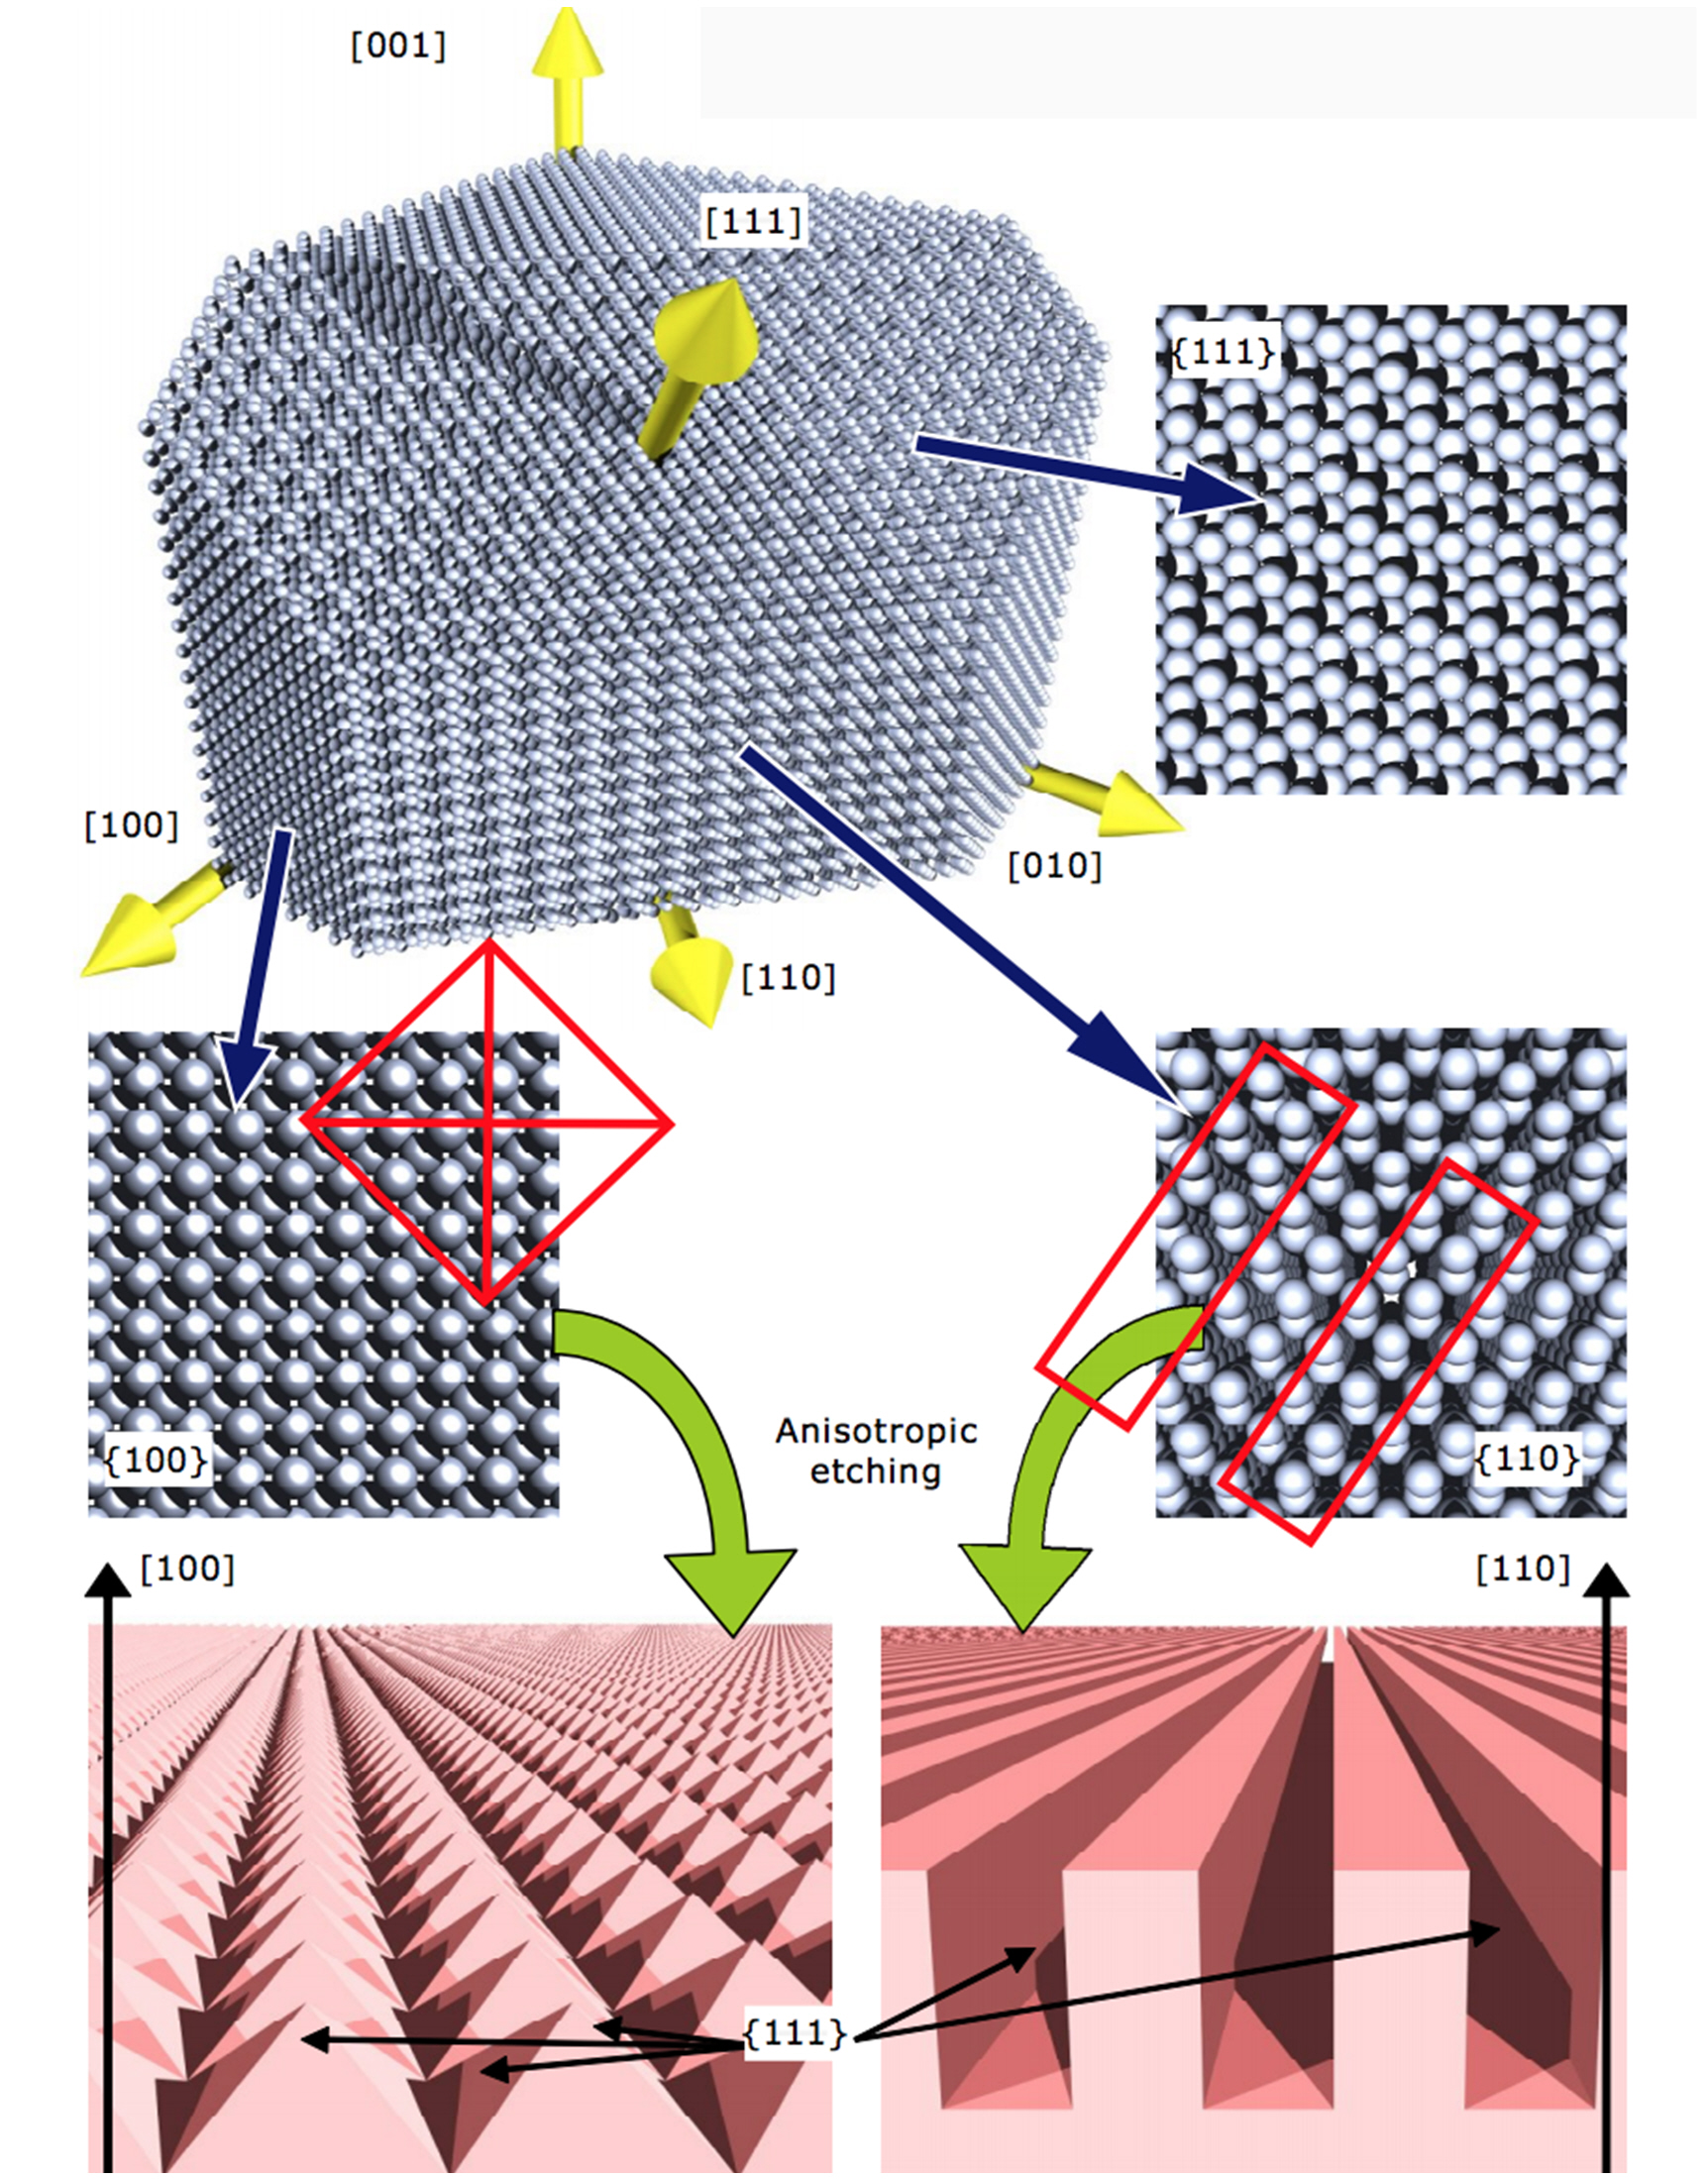
\includegraphics[width=12cm]{./Pictures/color_silicon_crystal.jpg}
	\captionsetup{justification=centering}
	\caption{硅的晶格结构及湿法腐蚀特性\cite{microchemicals}}
	\label{color_silicon_crystal}
\end{figure}

由于湿法腐蚀无法对SOI芯片均匀减薄,通常用来对SOI芯片减薄的方法有两种,一种是用ICP对较厚的SOI芯片进行刻蚀,这种方法的优势是工艺方便,缺点是表面会比较粗糙且厚度不均匀,会影响器件的损耗等性能,Zou等人采用该方法来减薄220~$nm$~SOI芯片得到60~$nm$厚的硅波导,损耗为0.61~dB/$cm$\cite{zou201560}。另一种方法是用热氧的方法氧化表面硅层之后用HF溶液去除氧化层,使得SOI芯片的硅层厚度减薄,Wang等人利用热氧化的方法制作了60~$nm$厚的硅波导,其波导损耗可以减小到0.35~dB/$cm$\cite{wang2017continuously}。相比较而言,利用热氧法进行硅层的减薄可以得到更低的损耗。

除了如图\ref{color_thin_application}中所示的一些器件需要将标准SOI芯片减薄,在许多常用硅基光电子器件制作测试时,我们也经常需要制作浅刻蚀的光栅耦合器方便器件的测试\cite{taillaert2004compact}。由于实验室的设备因为稳定性的原因,如果每次都通过制作测试片再用划台阶仪的方法来确定刻蚀速率或者氧化速率,则会增加工艺步骤,比较费时费力。这时如果有一种能够帮助我们快速确定薄硅层厚度的方法,就能给器件的工艺制作提供极大的便利。我们通过平时实验的经验发现,不同的刻蚀深度对应的SOI芯片颜色会有所不同。如图\ref{color_etch_time}所示,可以看到SOI芯片经过不同时间的ICP刻蚀,所剩下的不同厚度硅层显示出来的颜色信息非常丰富,硅层厚度为220~$nm$的SOI芯片没有刻蚀前显示为淡绿色,通过不同时间的刻蚀,会显示出紫色、黄色、蓝色等丰富的颜色,故我们对其进行了较为深入的研究,以期找出硅层厚度与颜色的对应关系。

\begin{figure}[htb]
	\centering
	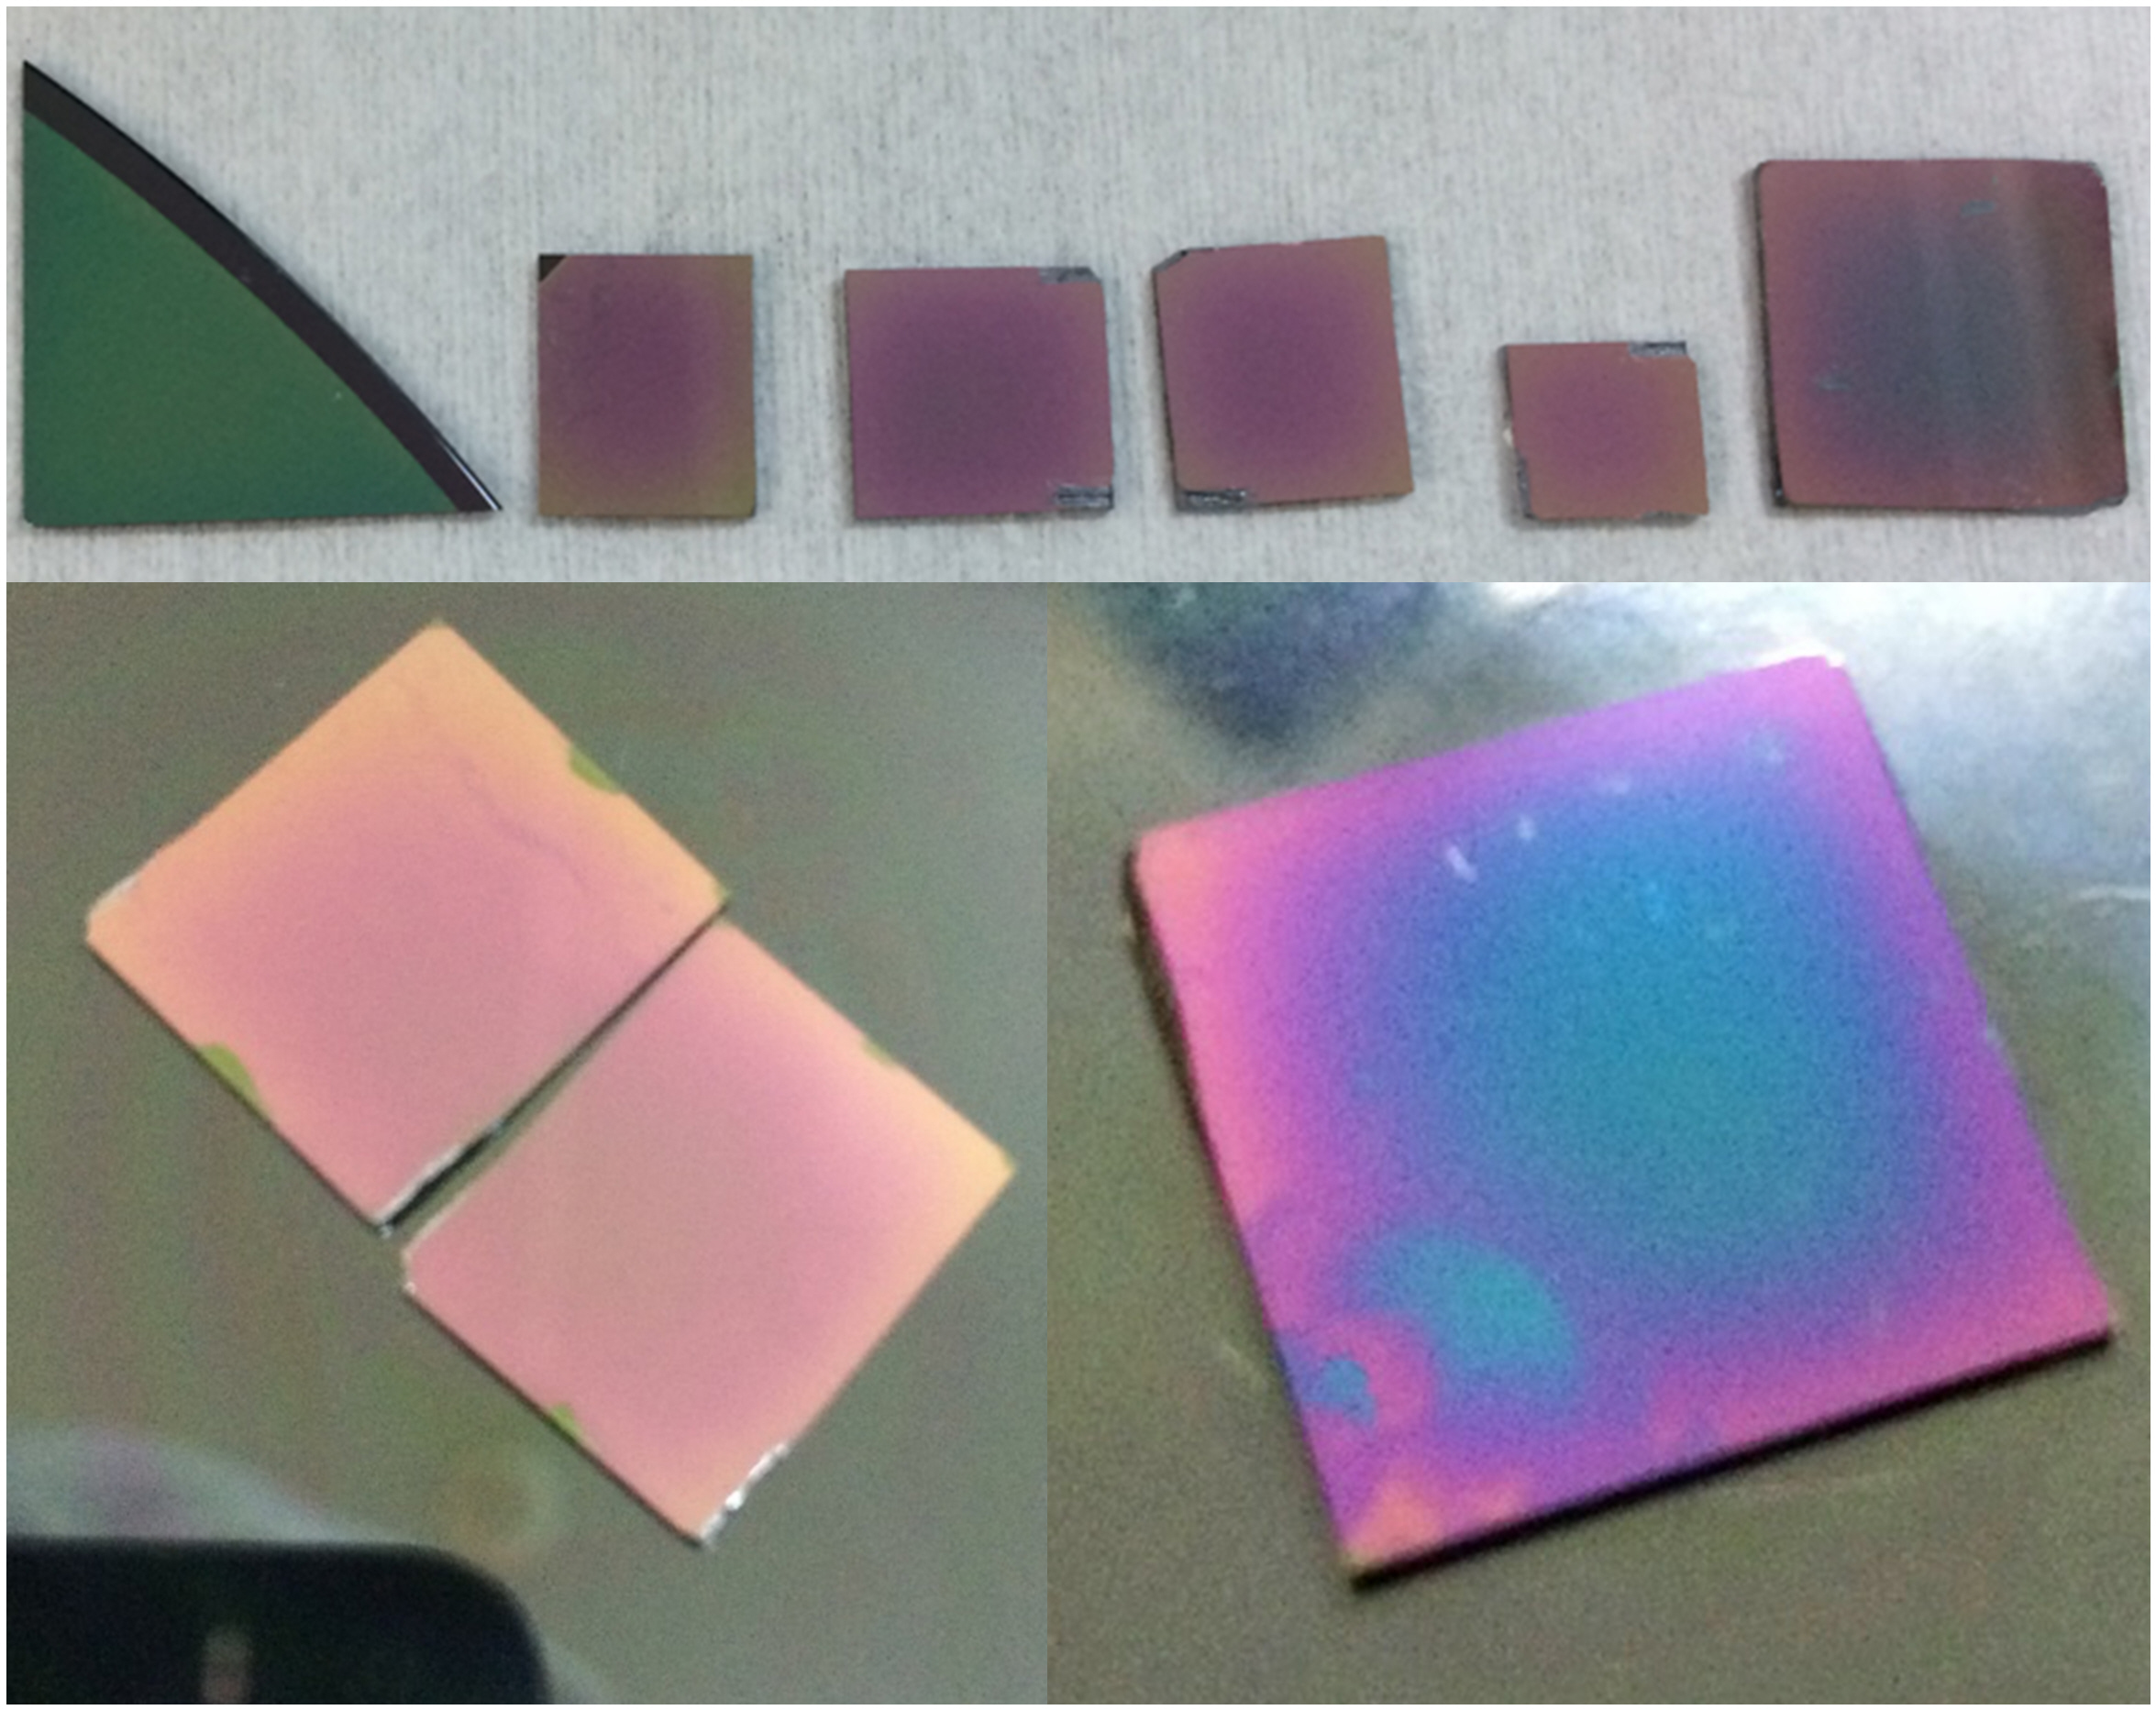
\includegraphics[width=12cm]{./Pictures/color_etch_time.jpg}
	\captionsetup{justification=centering}
	\caption{不同刻蚀深度对应的SOI的颜色}
	\label{color_etch_time}
\end{figure}

\section{光度学与色度学基础}
为了研究跟颜色相关的问题,我们首先需要一些光度学与色度学的基础。光是一种电磁波,其波长范围覆盖从1~$nm$以下直到10\SP{3}~$km$,其辐射类型按能量从高到低包括$\gamma$射线、X射线、紫外线、可见光、红外线、微波、无线电等。在整个电磁波谱中,只有很小的一部分进入人眼之后能引起我们的视觉感知,这部分光辐射谱被称为可见光谱,简称可见光。一般认为可见光的波长范围在380~$nm$\~{}780~$nm$之间,我们人眼所能够感知到的颜色都只与这个波长范围内的电磁波有关。不同波长的可见光辐射进入人眼,引起不同的颜色感觉,单一波长的可见光表现为一种颜色,称为单色光或者光谱色。

除了激光之外,日常生活中见到单色光的机会并不多,一般接触到的都是复色光。复色光中不同波长的单色光的相对功率分布决定了我们对它的颜色感觉。所以,成分确定的复色光一定对应一种确定的颜色。但是,一种确定的颜色并不只对应一种光谱组合,即两种不同的成分组合的复色光可以引起我们相同的颜色感觉,这在颜色科学中就是很重要的同色异谱问题。在我们之后的研究中也可以发现,不同硅层厚度可能对应相同的颜色。

要确定一个物体的颜色,我们就需要确定该物体在可见光波段所发射的光谱。如果该物体是光源,那么我们只需要知道该光源的发射谱;如果该物体本身并不发光,我们就需要确定光源的光谱,以及该物体对不同波长的光的反射率或者透射率,从而确定我们观察到该物体的光谱,之后就能确定该物体的颜色。

可见光在380~$nm$\~{}780~$nm$波长范围内的电磁辐射能量,可以用辐射量来描述,但是可见光对人的视觉形成刺激的程度不仅与电磁辐射的能量有关,还与人眼的响应有关,故我们需要用光学量(光度量)来描述其强弱。人们把定量地测定光的明亮程度的科学称为光度学(photometry)。辐射量是单位为焦耳($J$),瓦特($W$)等的物理量,而光学量是由视觉心理来评价物理量时得到的量,称为心理物理量,单位为流明($lm$),勒克斯($lx$)等。由此可见,当把可见光当做纯物理现象来研究时,应采用辐射量量值系统;当研究与人的视觉有关问题时,应采用光学量量值系统。为了后面讨论的方便,我们有必要介绍部分辐射量与光学量,以及两种量值之间的关系\cite{ydy2011gcgx,lxt2007jhgx}。

\subsection{辐射量}

\begin{enumerate}[(1)]
	\item
	辐射能$Q_{e}$~~~~同其他电磁辐射一样,可见光辐射也是一种能量传播形式。以电磁辐射形式发射、传输或接收的能量称为辐射能,通常用字符$Q_{e}$表示。度量辐射能的单位为焦[耳]($J$)。
	\item 
	辐射能通量$\Phi_{e}$~~~~单位时间内发射、传输或接收辐射能称之为辐射能通量,通常用字符$\Phi_{e}$表示。若在$dt$时间内发射、传输或接收的辐射能为d$Q_{e}$,相应的辐射能通量$\Phi_{e}$为:
	\begin{equation}
	\label{radiation_rate}
	\Phi_{e} = \dfrac{dQ_{e}}{dt}
	\end{equation}
	辐射能通量与功率有相同的单位,为瓦特($W$)。
	
\end{enumerate}
其他更多的辐射量由于跟本章内容无关,我们不再进行介绍。

\subsection{光学量}
\begin{enumerate}[]
	\item 
	光通量$\Phi_{v}$~~~~标度可见光对人眼的视觉刺激程度的量称为光通量,通常以字符$\Phi_{v}$表示。光通量的单位为流明($lm$)。
\end{enumerate}

其他更多的光学量量由于跟本章内容无关,我们不再进行介绍。

\begin{comment}
\begin{figure}[htb]
	\centering
	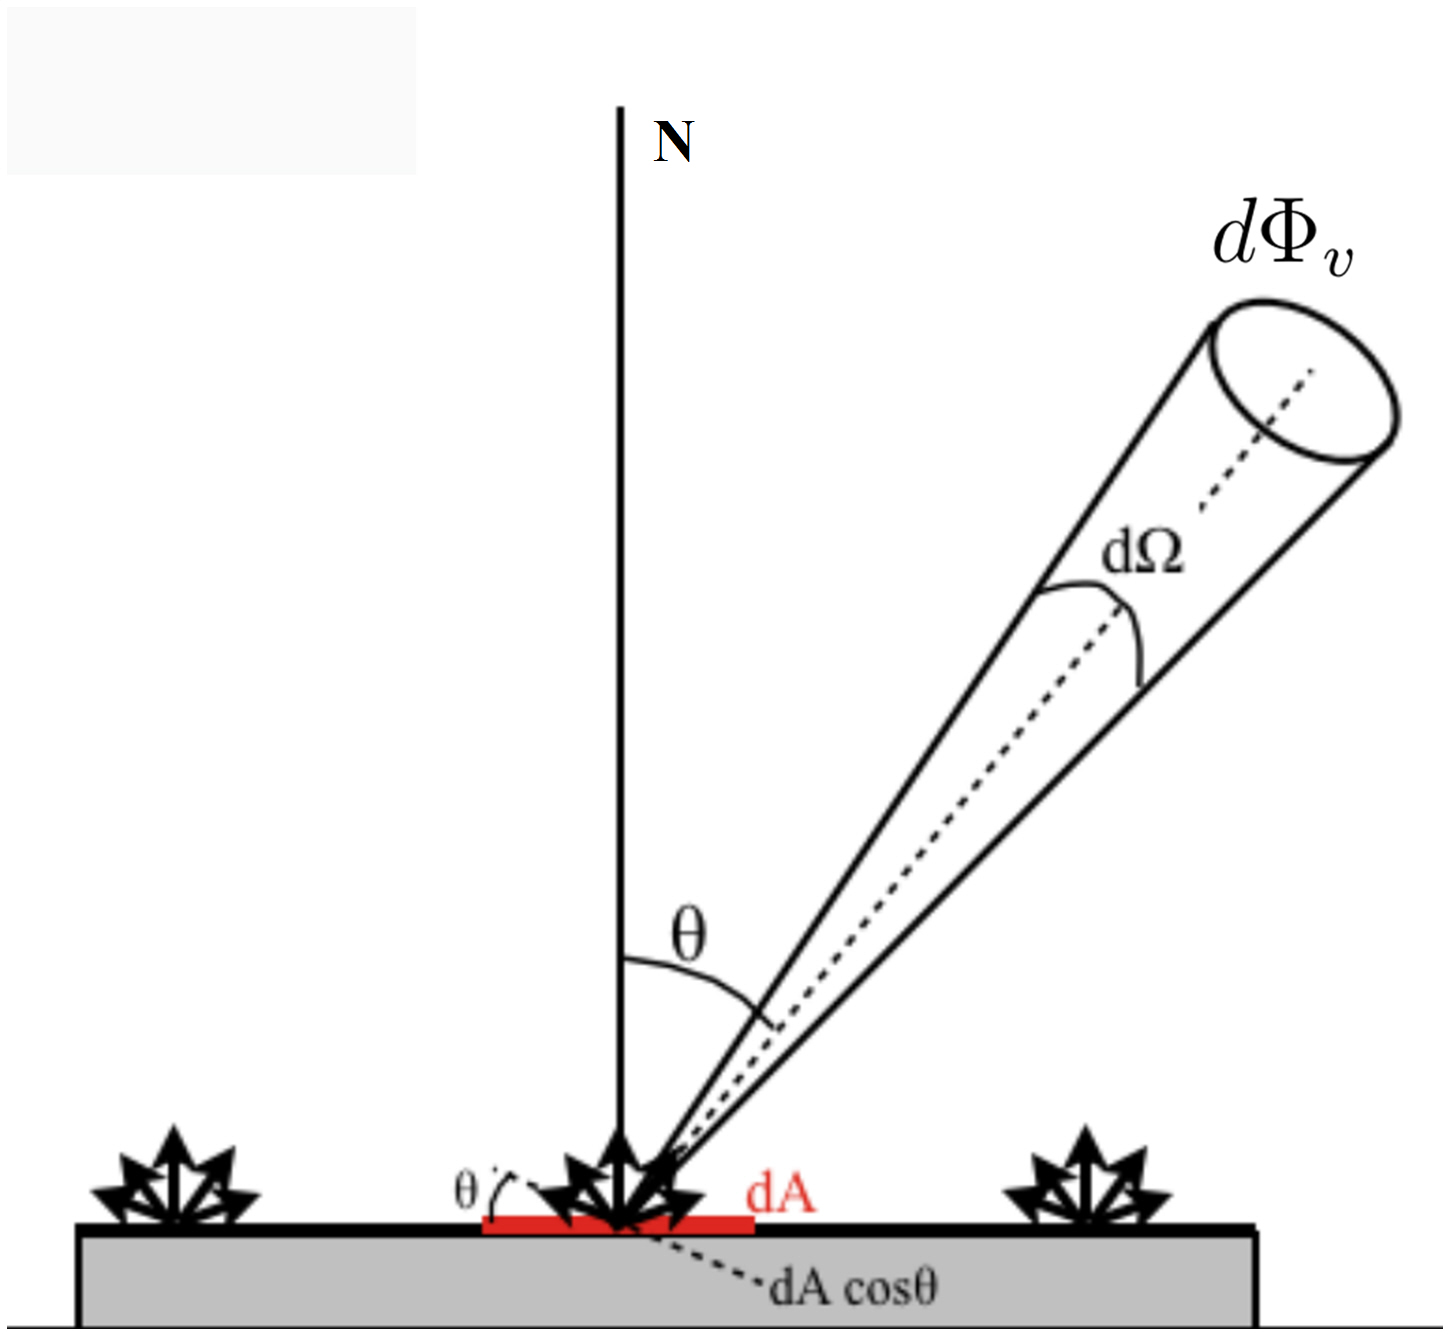
\includegraphics[width=12cm]{./Pictures/color_brightness.jpg}
	\captionsetup{justification=centering}
	\caption{光亮度定义示意图\cite{yalebrightness}}
	\label{color_brightness}
\end{figure}
\end{comment}

\subsection{光学量与辐射量之间的关系}
人的眼睛具有正确比较两个光刺激的强弱和判断其是否相等的能力,这是光度学的基础。但人眼对不同波长单色光的敏感程度并不一样,即相同功率的不同单色光所引起的光通量是不相同的。经过大量的实验确定,人眼对波长为555~$nm$的黄色光最为敏感,这正好是太阳辐射能量最高的波长附近。如果在单位波长内$P_{\lambda}$瓦的辐射能通量相当于$\Phi_{\lambda}$流明的光通量,则其比值:
\begin{equation}
\label{luminance_per_watt}
K_{\lambda} = \dfrac{\Phi_{\lambda}}{P_{\lambda}}
\end{equation}
可表示1瓦辐射能通量能量所相当的流明数。因为人眼对555~$nm$波长的黄光最为敏感,所以此数值在波长等于555~$nm$时取得最大。任一其他波长的单色光的$K_{\lambda}$值与$K_{555}$之比表征了人眼对该单色光辐射的相对灵敏度,称为光谱光视效率(spectral luminous efficiency)或视见函数(visibility function),以$V_{\lambda}$表示,即:
\begin{equation}
\label{visibility_function}
V_{\lambda} = \dfrac{K_{\lambda}}{K_{555}}
\end{equation}

\begin{figure}[htb]
	\centering
	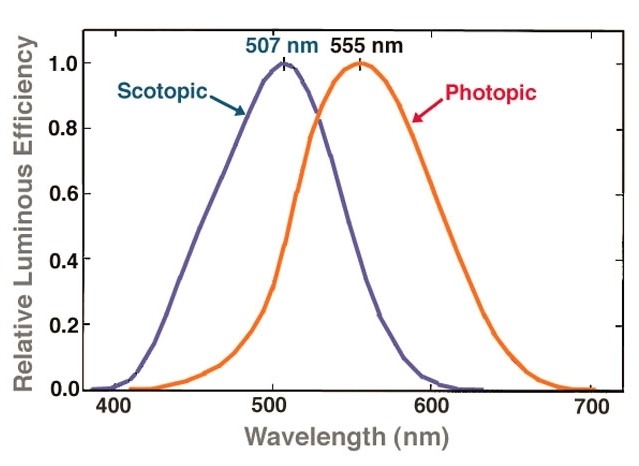
\includegraphics[width=11cm]{./Pictures/color_luminous_efficiency.jpg}
	\captionsetup{justification=centering}
	\caption{明场与暗场下相对光谱光视效率函数\cite{webvision}}
	\label{color_luminous_efficiency}
\end{figure}

不同波长单色光的光谱光视效率值是在做大量实验的基础上,由国际照明委员会(Commission Internationale de l´Eclairage, CIE)所确定的。实验表明,观察场明暗不同时,光谱光视效率亦稍有不同,这是由于人眼中的感光细胞分为视锥细胞和视杆细胞,视锥细胞工作在明视觉的情况下,可以感知颜色,但是灵敏度不如视杆细胞;视杆细胞工作在暗视觉的情况下,不能感知颜色,但是灵敏度很高。因此光谱光视效率函数在明暗场时略有不同,如图\ref{color_luminous_efficiency}所示,图中黄色曲线代表明场条件下的光谱光视效率函数,在555~$nm$处取得最大值,紫色曲线代表暗场(照度小于0.1~$lx$)\cite{hunt1995reproduction}条件下的光谱光视效率函数,在507~$nm$处取得最大值。在研究SOI芯片的硅层厚度与其颜色之间的对应关系时,我们只考虑明场的情况。

在波长$\lambda$附近的小波长间隔d$\lambda$内,光通量d$\Phi_{v}(\lambda)$和辐射能通量d$\Phi_{e}(\lambda)$之间的关系可以表示为:
\begin{equation}
\label{relation1}
d\Phi_{v}(\lambda)~=~K_{m}V(\lambda)\Phi_{e}(\lambda)d\lambda
\end{equation}
其中,$K_{m}$ = 683 $lm$/W为明视觉条件下波长为555~nm单色光的绝对光谱光视效率值;$K_{m}^{,}$ = 1755 lm/W为暗视觉条件下波长507~$nm$单色光的绝对光谱光视效率值。对于整个可见光谱范围内的总光通量$\Phi_{v}$,可由公式\ref{relation1}积分得到:
\begin{equation}
\label{relation3}
\Phi_{v}(\lambda)~=~\int_{380}^{780}K_{m}V(\lambda)\Phi_{e}(\lambda)d\lambda
\end{equation}

\subsection{CIE1931-RGB系统}
人们做了大量的颜色匹配实验,得出如下两个结论:
\begin{enumerate}[(1)]
	\item 
	红、绿、蓝三种颜色以不同的量值(有的可能为负值)相混合,可以匹配出任何颜色。
	\item 
	红、绿、蓝不是唯一的能匹配所有颜色的三种颜色。三种颜色,只要其中的每一种都不能用其他两种混合产生出来,就可以用它们匹配所有的颜色。
\end{enumerate}

我们将能够匹配所有颜色的三种颜色称为三原色。在颜色匹配中,以一定数量的三原色能够完成某种颜色的匹配,匹配某种颜色所需的三原色称作该颜色的三刺激值。三刺激值一般不用物理单位而需要用色度学的单位来度量。

如果用红、绿、蓝三原色匹配等能光谱色所需的量称为光谱三刺激值,等能光谱是指各波长辐射能量相等,只有在此条件下,所得到的光谱三刺激值才是可比较和有意义的。对于不用波长的光谱色,其三刺激值显然为波长$\lambda$的函数,故也可以称为颜色匹配函数,一般用$\overline{r}(\lambda)$、$\overline{g}(\lambda)$和$\overline{b}(\lambda)$表示。可以用方程表示为:
\begin{equation}
\label{guangpuse}
C(\lambda)\equiv\overline{r}(\lambda)+\overline{g}(\lambda)+\overline{b}(\lambda)
\end{equation}
式中,$\equiv$表示两边的颜色匹配,显示相同的颜色,该类方程也被称为颜色方程。颜色匹配函数如图\ref{color_rgb_combined}(a)所示,他是将物理刺激与人体生理响应结合起来的纽带。从图中可以看出,红色刺激值就有可能是负值。

\begin{figure}[htb]
	\centering
	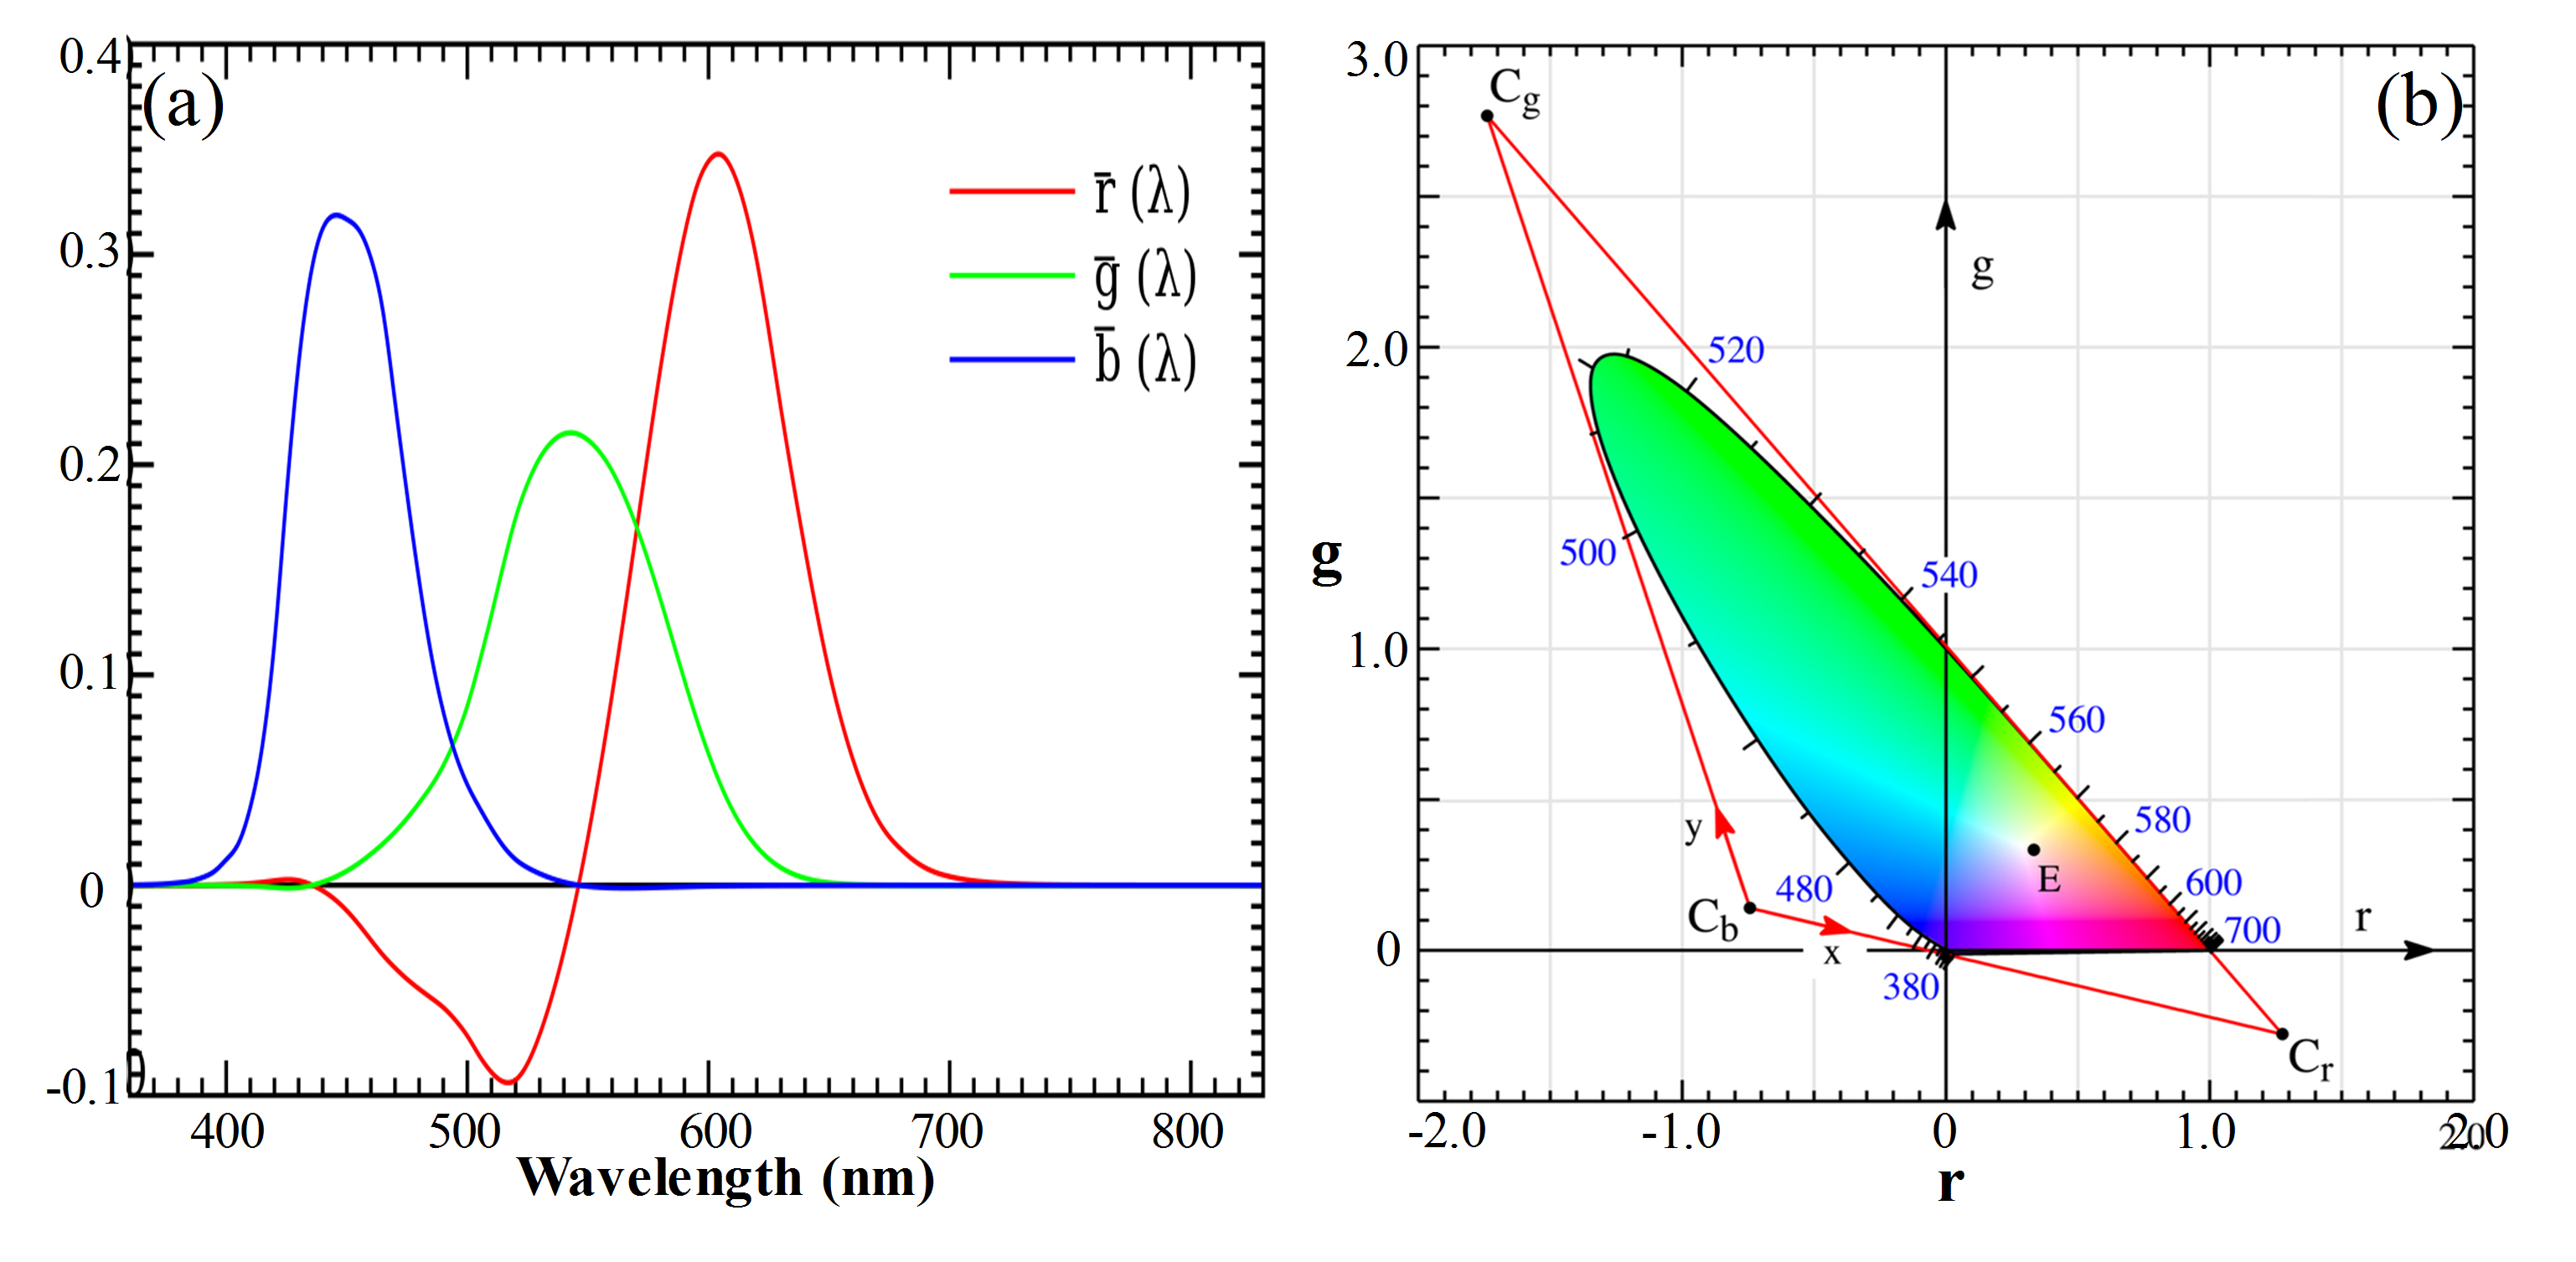
\includegraphics[width=16cm]{./Pictures/color_rgb_combined.jpg}
	\captionsetup{justification=centering}
	\caption{(a)~CIE1931~RGB色度系统光谱三刺激值曲线;(b)~CIE1931~RGB色品图\cite{wikicie1931}}
	\label{color_rgb_combined}
\end{figure}

在颜色研究和度量中,一般不用颜色的三刺激值R、G、B来表示颜色,而是用三刺激值各自在三刺激总量R+G+B中所占的比例来表示颜色,也叫做色品。选用R、G、B为三原色时,用r、g、b来表示色品坐标,有:
\begin{equation}
\label{sepin}
r=\dfrac{R}{R+G+B};~g=\dfrac{G}{R+G+B};~b=\dfrac{B}{R+G+B}
\end{equation}
且r~+~g~+~b~=~1。当计算光谱色的色品坐标时,只需要将R、G、B替换为$\overline{r}(\lambda)\mbox{、}\overline{g}(\lambda)\mbox{、}\overline{b}(\lambda)$即可,结果如图\ref{color_rgb_combined}(b)所示,图中马蹄形曲线为光谱色色品点轨迹,从图中给我们可以发现有的颜色的色品坐标是负的,这既不便于计算,也难于理解,因此CIE同时推荐了另一色度学系统,即CIE1931-XYZ系统。

\subsection{CIE1931-XYZ系统}
CIE1931-XYZ系统选用了X、Y、Z为三原色,该三原色的选取遵循规则如下:
\begin{enumerate}[(1)]
	\item 
	用此三原色匹配等能光谱色,三刺激值不应出现负值。
	\item 
	实际不存在的颜色在色品图上所占的面积应尽量小。
	\item 
	用Y刺激值表示颜色的亮度,同时亦表示色度;而X和Z刺激值只表示色度,不代表亮度。
\end{enumerate}

根据以上原则,求出X、Y、Z三原色在CIE1931-RGB中的色品坐标如表\ref{coordinate_XYZ}所示,此时X、Y、Z三原色并不实际存在,只是3个虚拟的颜色,故不能用来进行配色实验得到三刺激值曲线。CIE根据RGB的三刺激曲线经过坐标转换和定标,得到CIE1931XYZ系统下的三刺激值曲线,也叫CIE1931标准色度观察者光谱三刺激值曲线,如图\ref{color_xyz_combined}(a)所示。从中可以看出,刺激值已经没有负值。

\begin{table}[htb]
	\zihao{5}
	\captionsetup{justification=centering}
	\caption{XYZ三原色在RGB系统中的色品坐标}
	\label{coordinate_XYZ}
	\centering
	\begin{tabular}[t]{|cccc|}
		\hline
		& r & g & b  \\
		\hline
		(X) & 1.2750 & -0.2778 & 0.0028  \\
		\hline
		(Y)	& -1.7392 & 2.7671 & -0.0279  \\
		\hline
		(Z)	& -0.7431 & 0.1409 & 1.6022  \\
		\hline
	\end{tabular}
\end{table}

\begin{figure}[htb]
	\centering
	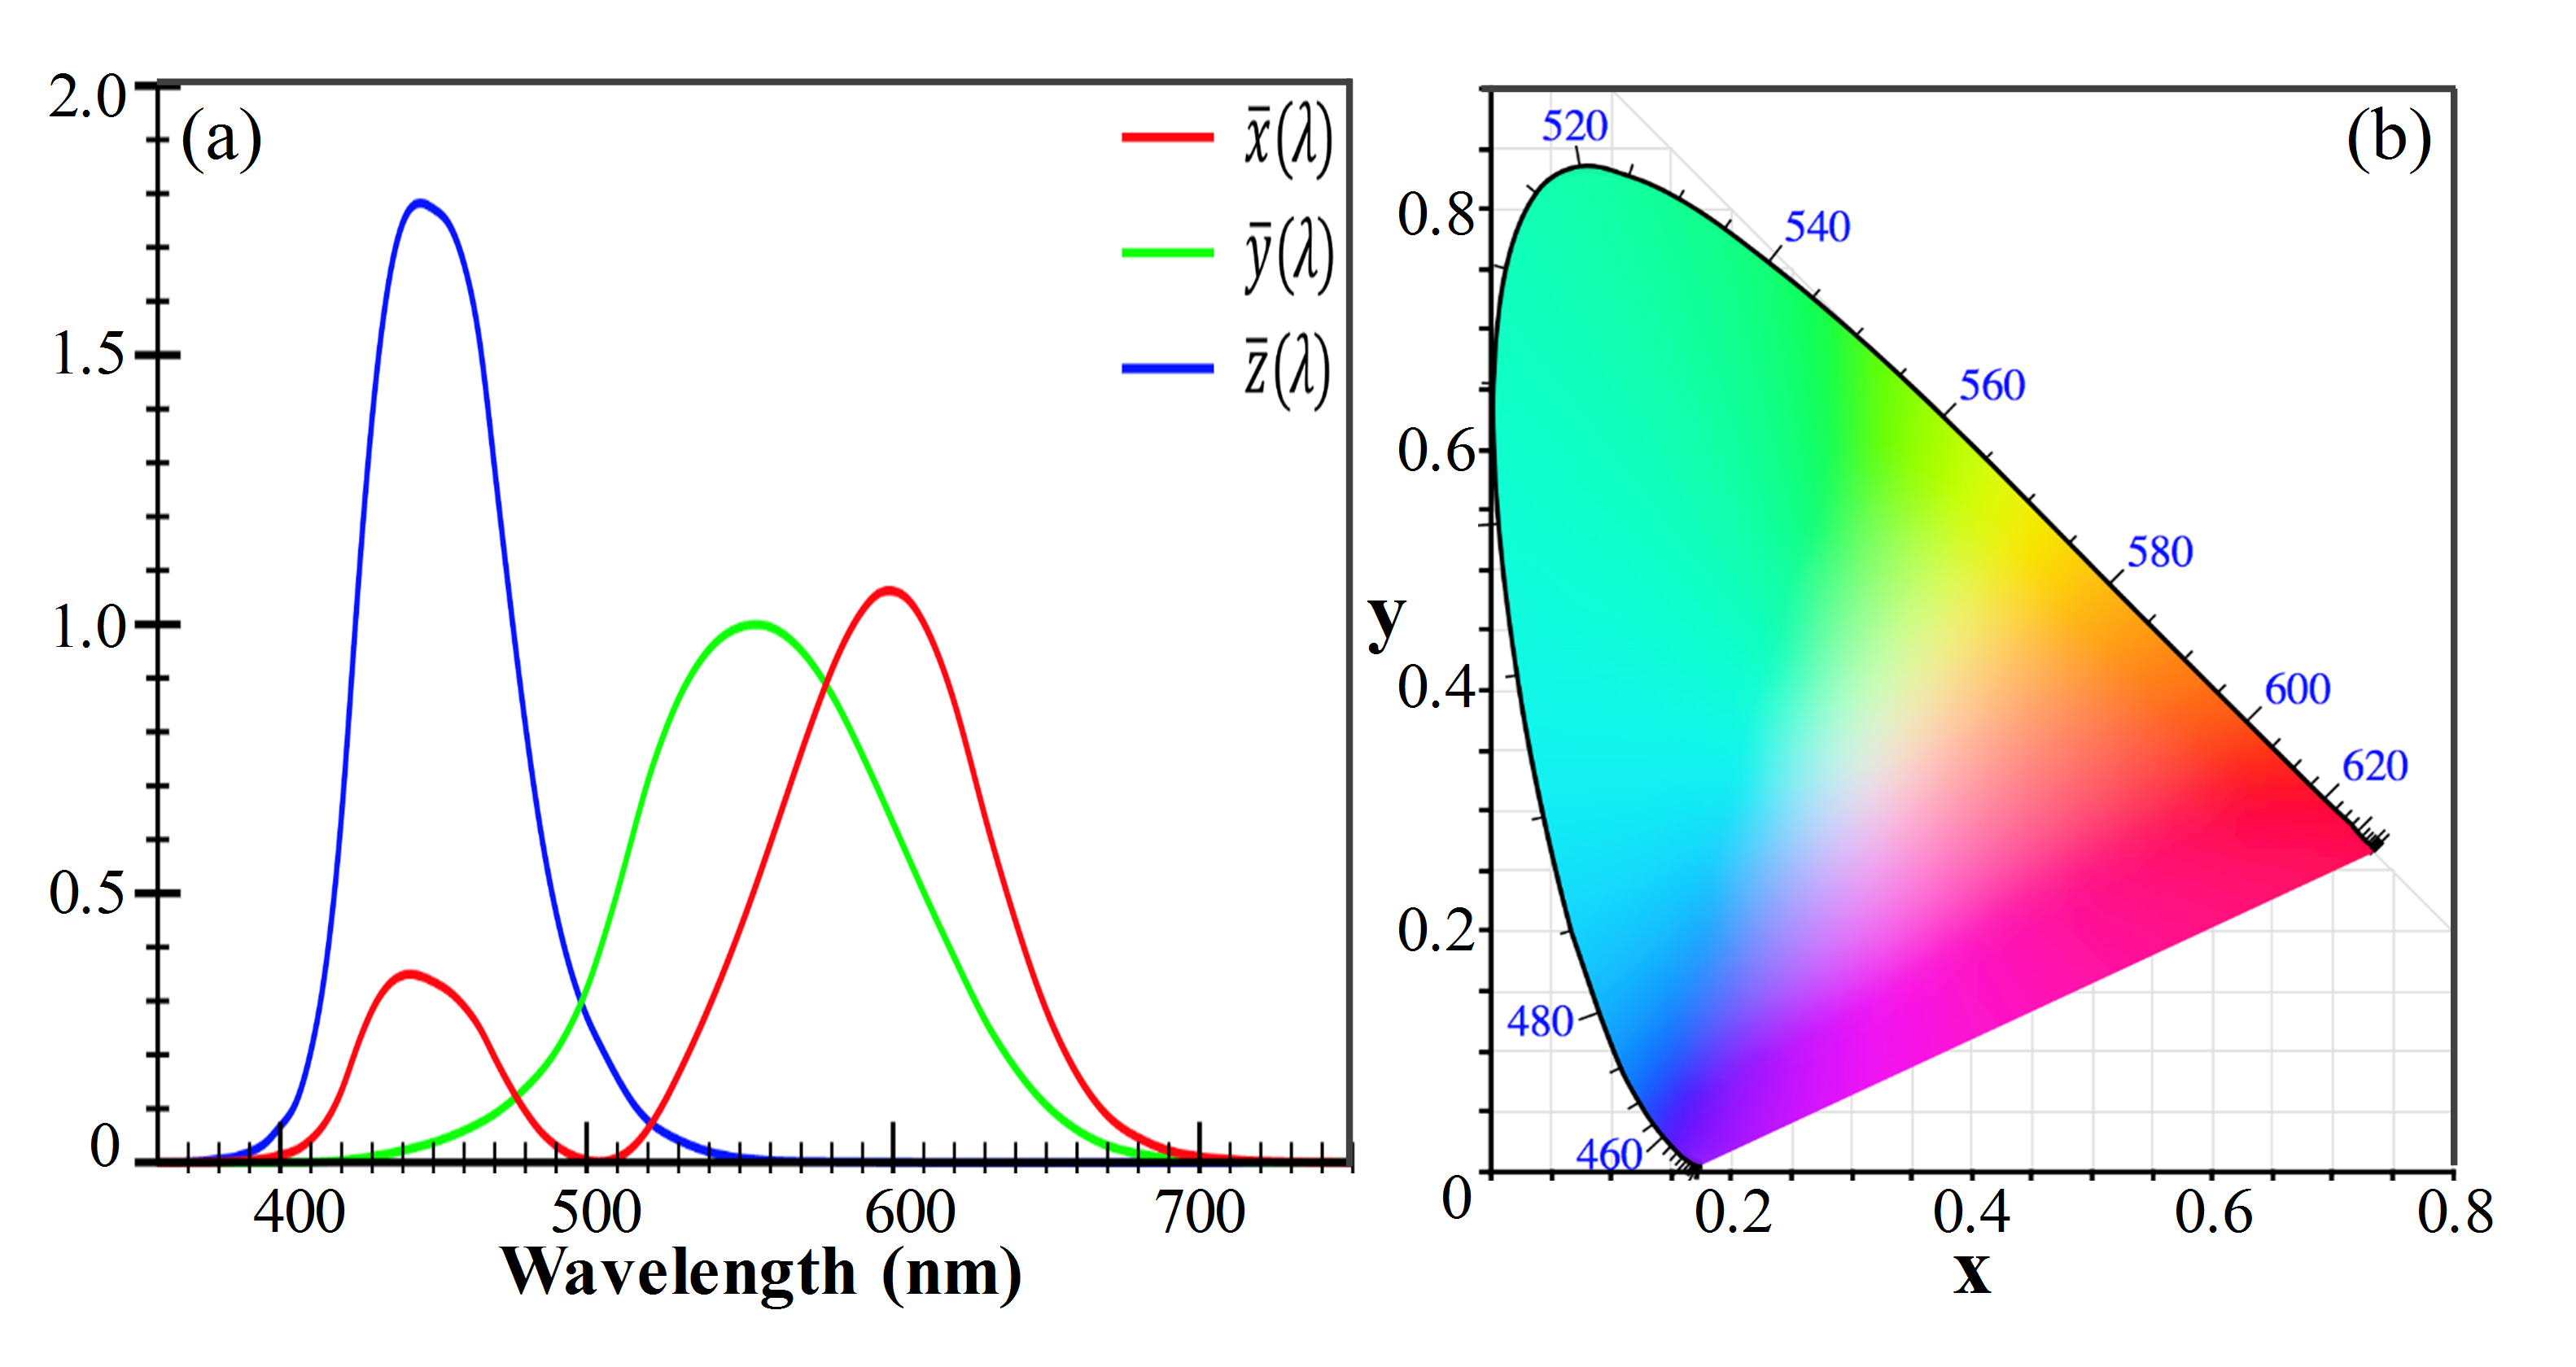
\includegraphics[width=16cm]{./Pictures/color_xyz_combined.jpg}
	\captionsetup{justification=centering}
	\caption{(a)~CIE1931~XYZ色度系统光谱三刺激值曲线;(b)~CIE1931~XYZ色品图\cite{wikicie1931}}
	\label{color_xyz_combined}
\end{figure}

与CIE1931-RGB系统类似,我们也可定义CIE1931-XYZ系统的色品坐标为:
\begin{equation}
\label{sepin_XYZ}
x=\dfrac{X}{X+Y+Z};~y=\dfrac{Y}{X+Y+Z};~z=\dfrac{Z}{X+Y+Z}
\end{equation}
且x~+~y~+~z~=~1。据此得到CIE1931色品图,如图\ref{color_xyz_combined}(b)所示。


至此,如果我们已知颜色刺激的波长分布$\varphi(\lambda)$,即不同波长上的辐射能通量,我们就可以根据公式\ref{stimulate_X}\~{}\ref{stimulate_Z}求得颜色的三刺激值,以及色品坐标。

\begin{equation}
\label{stimulate_X}
X=k\int_{380}^{780}\varphi(\lambda)\overline{x}(\lambda)d\lambda
\end{equation}
\begin{equation}
\label{stimulate_Y}
Y=k\int_{380}^{780}\varphi(\lambda)\overline{y}(\lambda)d\lambda
\end{equation}
\begin{equation}
\label{stimulate_Z}
Z=k\int_{380}^{780}\varphi(\lambda)\overline{z}(\lambda)d\lambda
\end{equation}
其中$k=\dfrac{100}{Y}$,因为CIE规定Y刺激值为1或者100,为显示设备支持的最亮的白色。由于$\overline{x}(\lambda)$、$\overline{y}(\lambda)$、$\overline{z}(\lambda)$等参数常常以一定波长间隔的离散形式给出,所以在实际计算时,常常用求和的方式代替积分。

\subsection{CIE-XYZ坐标转换为CIE-RGB坐标}
由XYZ色坐标系统的定义可知,其为RGB系统的线性变换。我们采用sRGB来表示最后计算得到的颜色,sRGB为RGB的一种,其三原色的xyz坐标点如表\ref{sRGBxyz}所示。然后可以用公式\ref{XYZ2RGB}\cite{international1999iec}将XYZ刺激值转换为RGB三刺激值,再得出rgb色品坐标。
\begin{table}[htb]
	\zihao{5}
	\captionsetup{justification=centering}
	\caption{sRGB三原色与参考白xyY坐标点}
	\label{sRGBxyz}
	\centering
	\begin{tabular}[t]{|ccccc|}
		\hline
		& Red & Green & Blue & White point \\
		\hline
		x & 0.6400 & 0.3000 & 0.1500 & 0.3127 \\
		\hline
		y	& 0.3300 & 0.6000 & 0.0600 & 0.3290 \\
		\hline
		Y	& 0.2126 & 0.7152 & 0.0722 & 1.0000 \\
		\hline
	\end{tabular}
\end{table}

\begin{equation}
\label{XYZ2RGB}
\left[\begin{array}{c}
R\\
G\\
B
\end{array}
\right]=
\begin{bmatrix}
3.2406 & -1.5372 & -0.4986\\
-0.9689 & 1.8758 & 0.0415\\
0.0557 & -0.2040 & 1.570
\end{bmatrix}
\begin{bmatrix}
X\\Y\\Z
\end{bmatrix}
\end{equation}

由于显示器的亮度显示是非线性的,我们还需用公式\ref{gamma}对所得的rgb值进行伽马校正\cite{international1999iec}。

\begin{equation}
\label{gamma}
c_{srgb} = \left\{
\begin{array}{lcc}
12.92c_{rgb}, &     & c_{rgb}\le0.0031308\\
(1+a)c_{rgb}^{1/2.4}-a,&     & c_{rgb}>0.0031308
\end{array}
	\right.
\end{equation}
其中a~=~0.055,c表示r、g或者b坐标。

至此,我们就可以根据光谱先计算得到XYZ三刺激值,利用转换矩阵得到RGB三刺激值,然后得到rgb色品坐标,经过伽马校正之后,我们就可以得到最终颜色的rgb值。

\section{SOI色谱图的计算}
我们采用Lumerical FDTD Solutions\cite{fdtdsolution}来仿真硅薄层的反射率,仿真模型如图\ref{color_reflection}(a)所示。图\ref{color_reflection}(b)显示了150~$nm$硅层厚度下,不同波长的光的反射率,从中可以明显看出薄膜干涉现象,而且因为硅在可见光波段具有明显的吸收,该反射谱还包含了吸收的信息。具体建模过程描述如下:

\begin{figure}[htb]
	\centering
	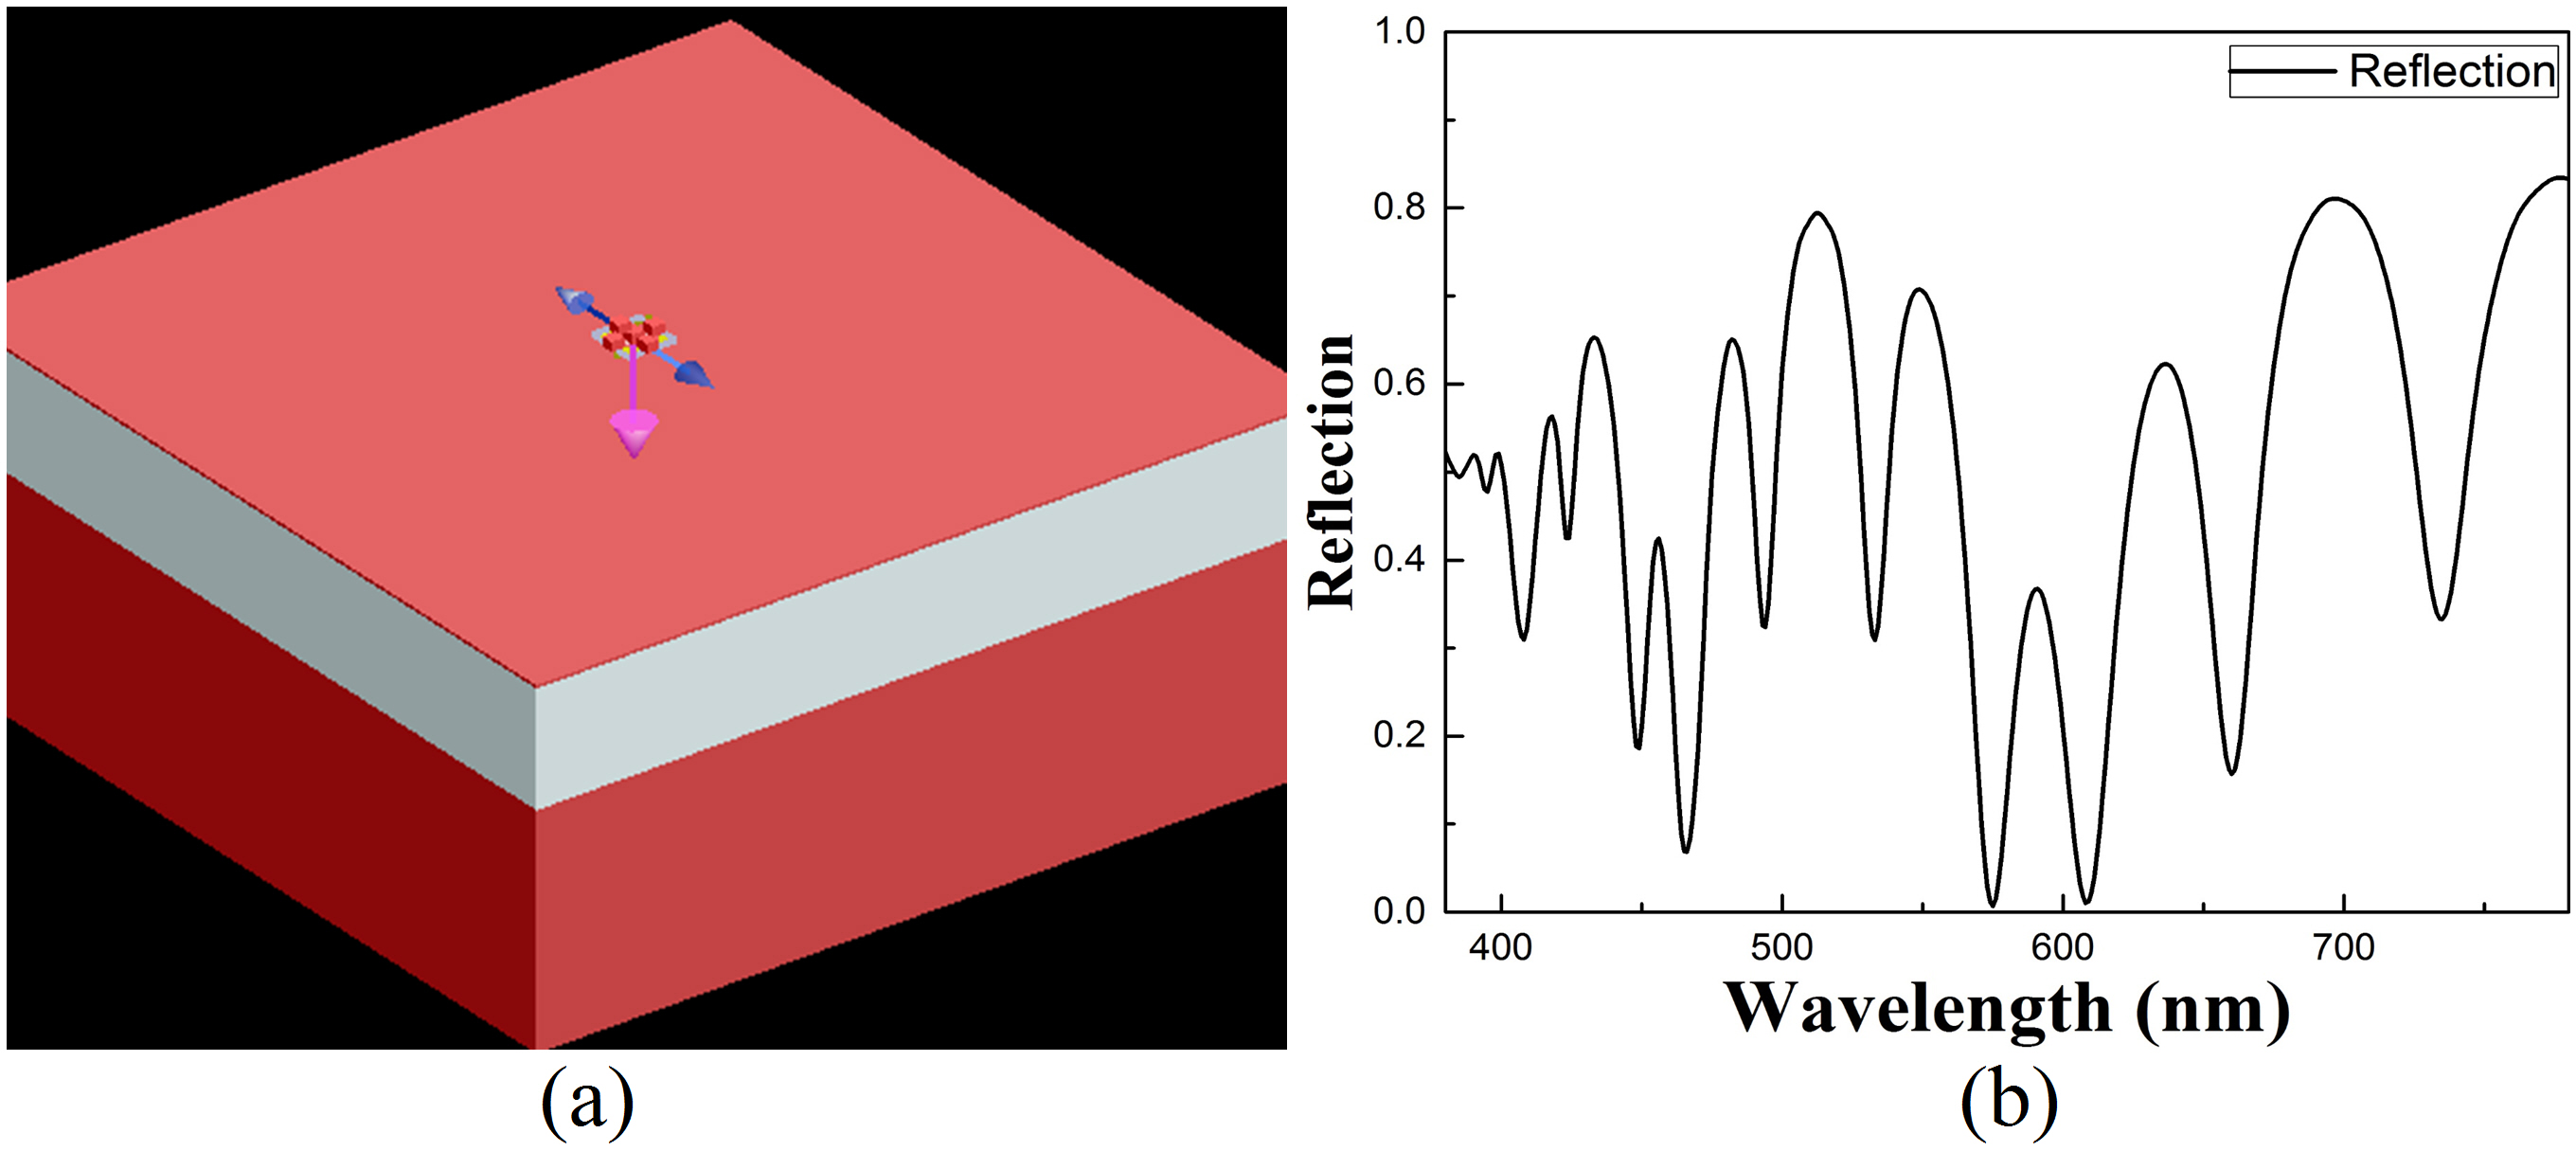
\includegraphics[width=14cm]{./Pictures/color_reflection.jpg}
	\captionsetup{justification=centering}
	\caption{SOI硅薄层(a)仿真模型;(b)仿真得到150~$nm$硅层厚度的反射率}
	\label{color_reflection}
\end{figure}

\begin{enumerate}[(1)]
	\item 
	仿真结构的建立与材料的选取:仿真的结构是基于实际SOI平芯片设置,衬底设为硅,二氧化硅氧化层的厚度为2~$\mu m$,硅层厚度扫描从0~\~{}~220~$nm$,上包层为空气。材料折射率采用软件内部使用的Palik测定值。
	\item 
	FDTD仿真区域与边界条件的设置:结构确定之后需要设置仿真区域,采用3D FDTD进行仿真,当硅层厚度比较薄时,光可以穿透硅层到达衬底,故我们将仿真区域延伸到衬底当中。边界条件的设置:在水平方向上设置为周期边界条件,来模拟无穷大的硅层。上下边界条件设为完美匹配层(Perfectly matched layer, PML)来模拟无穷大的空间。
	\item 
	仿真光源的选取:假设我们在日光下观察SOI芯片,故仿真中我们用平面光源来模拟实际情况。仿真的波长范围设置为380~\~{}~780~$nm$。
	\item 
	求解区域的网格划分:根据第二章中对时域有限差分方法的描述,在仿真计算过程中需要对求解区域进行网格划分,我们采用软件提供的自适应网格技术对网格进行划分,划分精度为3,如图\ref{color_mesh}所示。可以看到在硅层,因为折射率较高,所以网格划分也较为致密。
	\begin{figure}[htb]
		\centering
		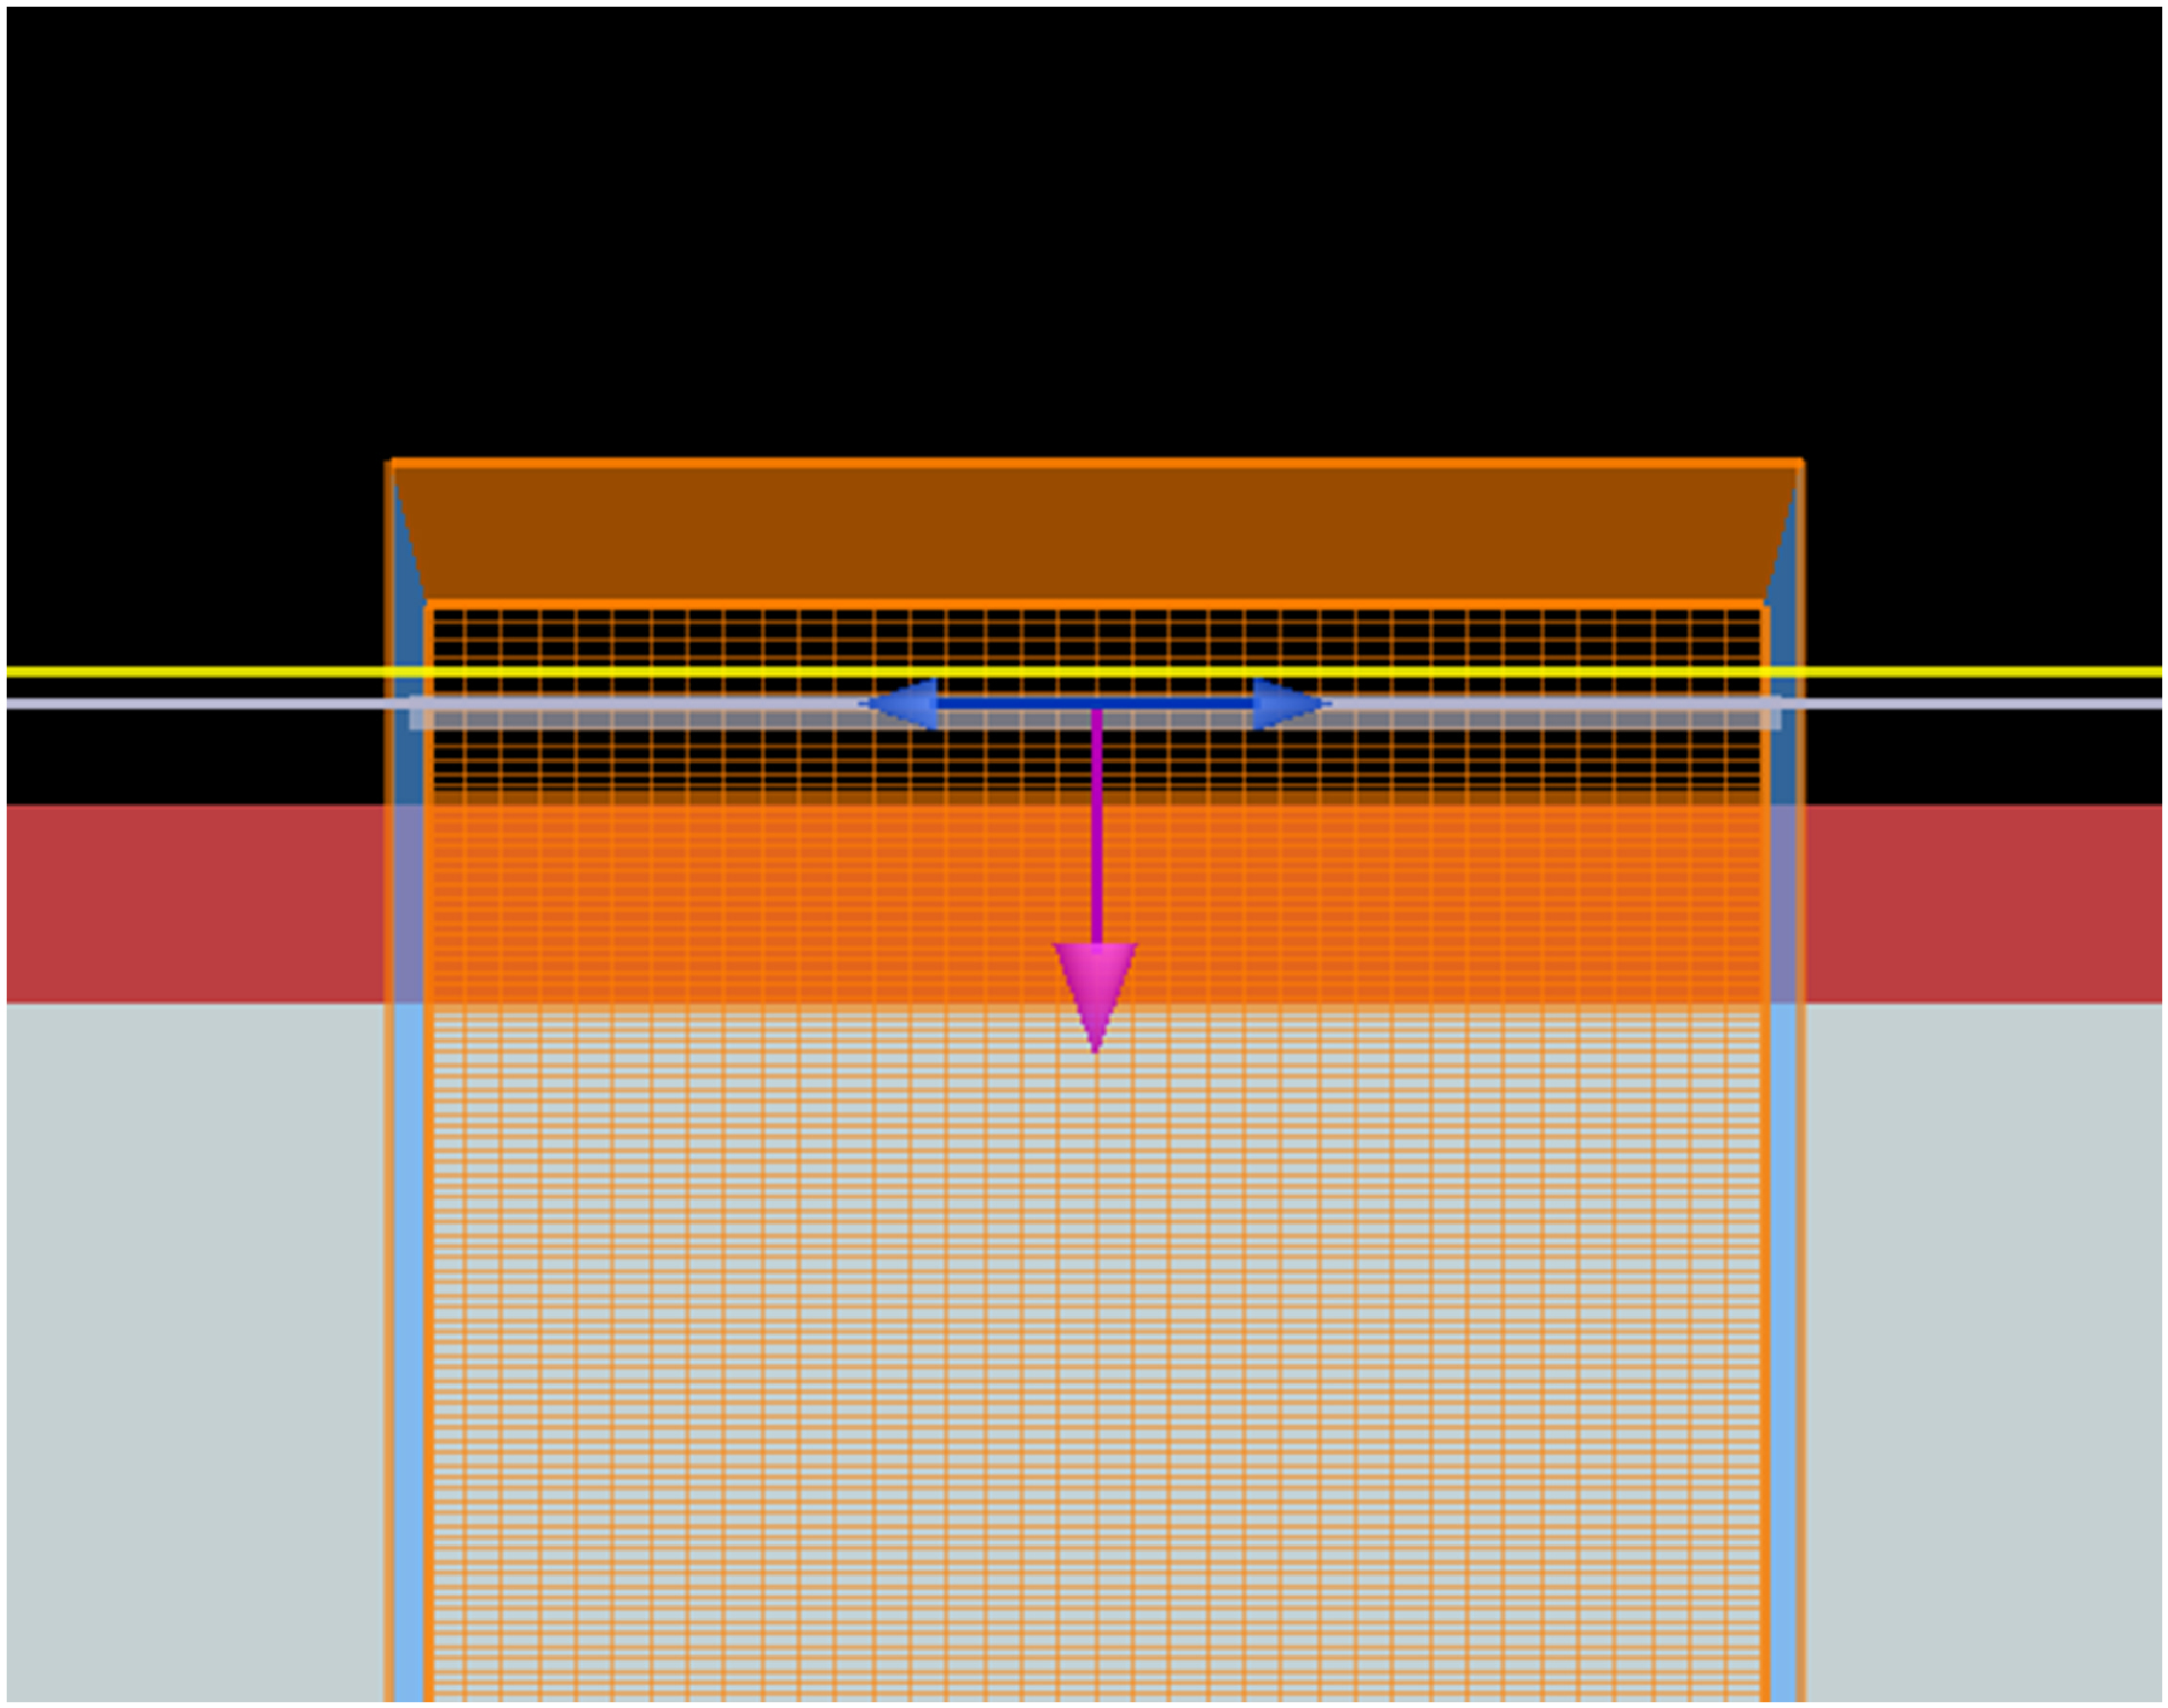
\includegraphics[width=10cm]{./Pictures/color_mesh.jpg}
		\captionsetup{justification=centering}
		\caption{FDTD solutions仿真区域网格划分}
		\label{color_mesh}
	\end{figure}
	\item 
	功率监视器的设置:将功率监视器放置于光源上方来观察结构在不同波长入射光下的反射特性。
\end{enumerate}

用上述模型扫描SOI不同硅层厚度时的反射谱,我们得到图\ref{color_reflection_all}所示的结果.图中横坐标表示不同的波长,纵坐标为硅层的厚度,所以每一条横线表示某个硅层厚度下的反射谱。我们可以看到当硅层厚度较小时,短波长处的谐振峰强度较大,随着硅层厚度的增大,其强度慢慢减弱,可以预测当硅层厚度较小时,蓝色会比较明显。我们还可以看到当硅层厚度变化时,谐振峰的漂移较为连续,故应可以得到较为连续的颜色变化。

\begin{figure}[htb]
	\centering
	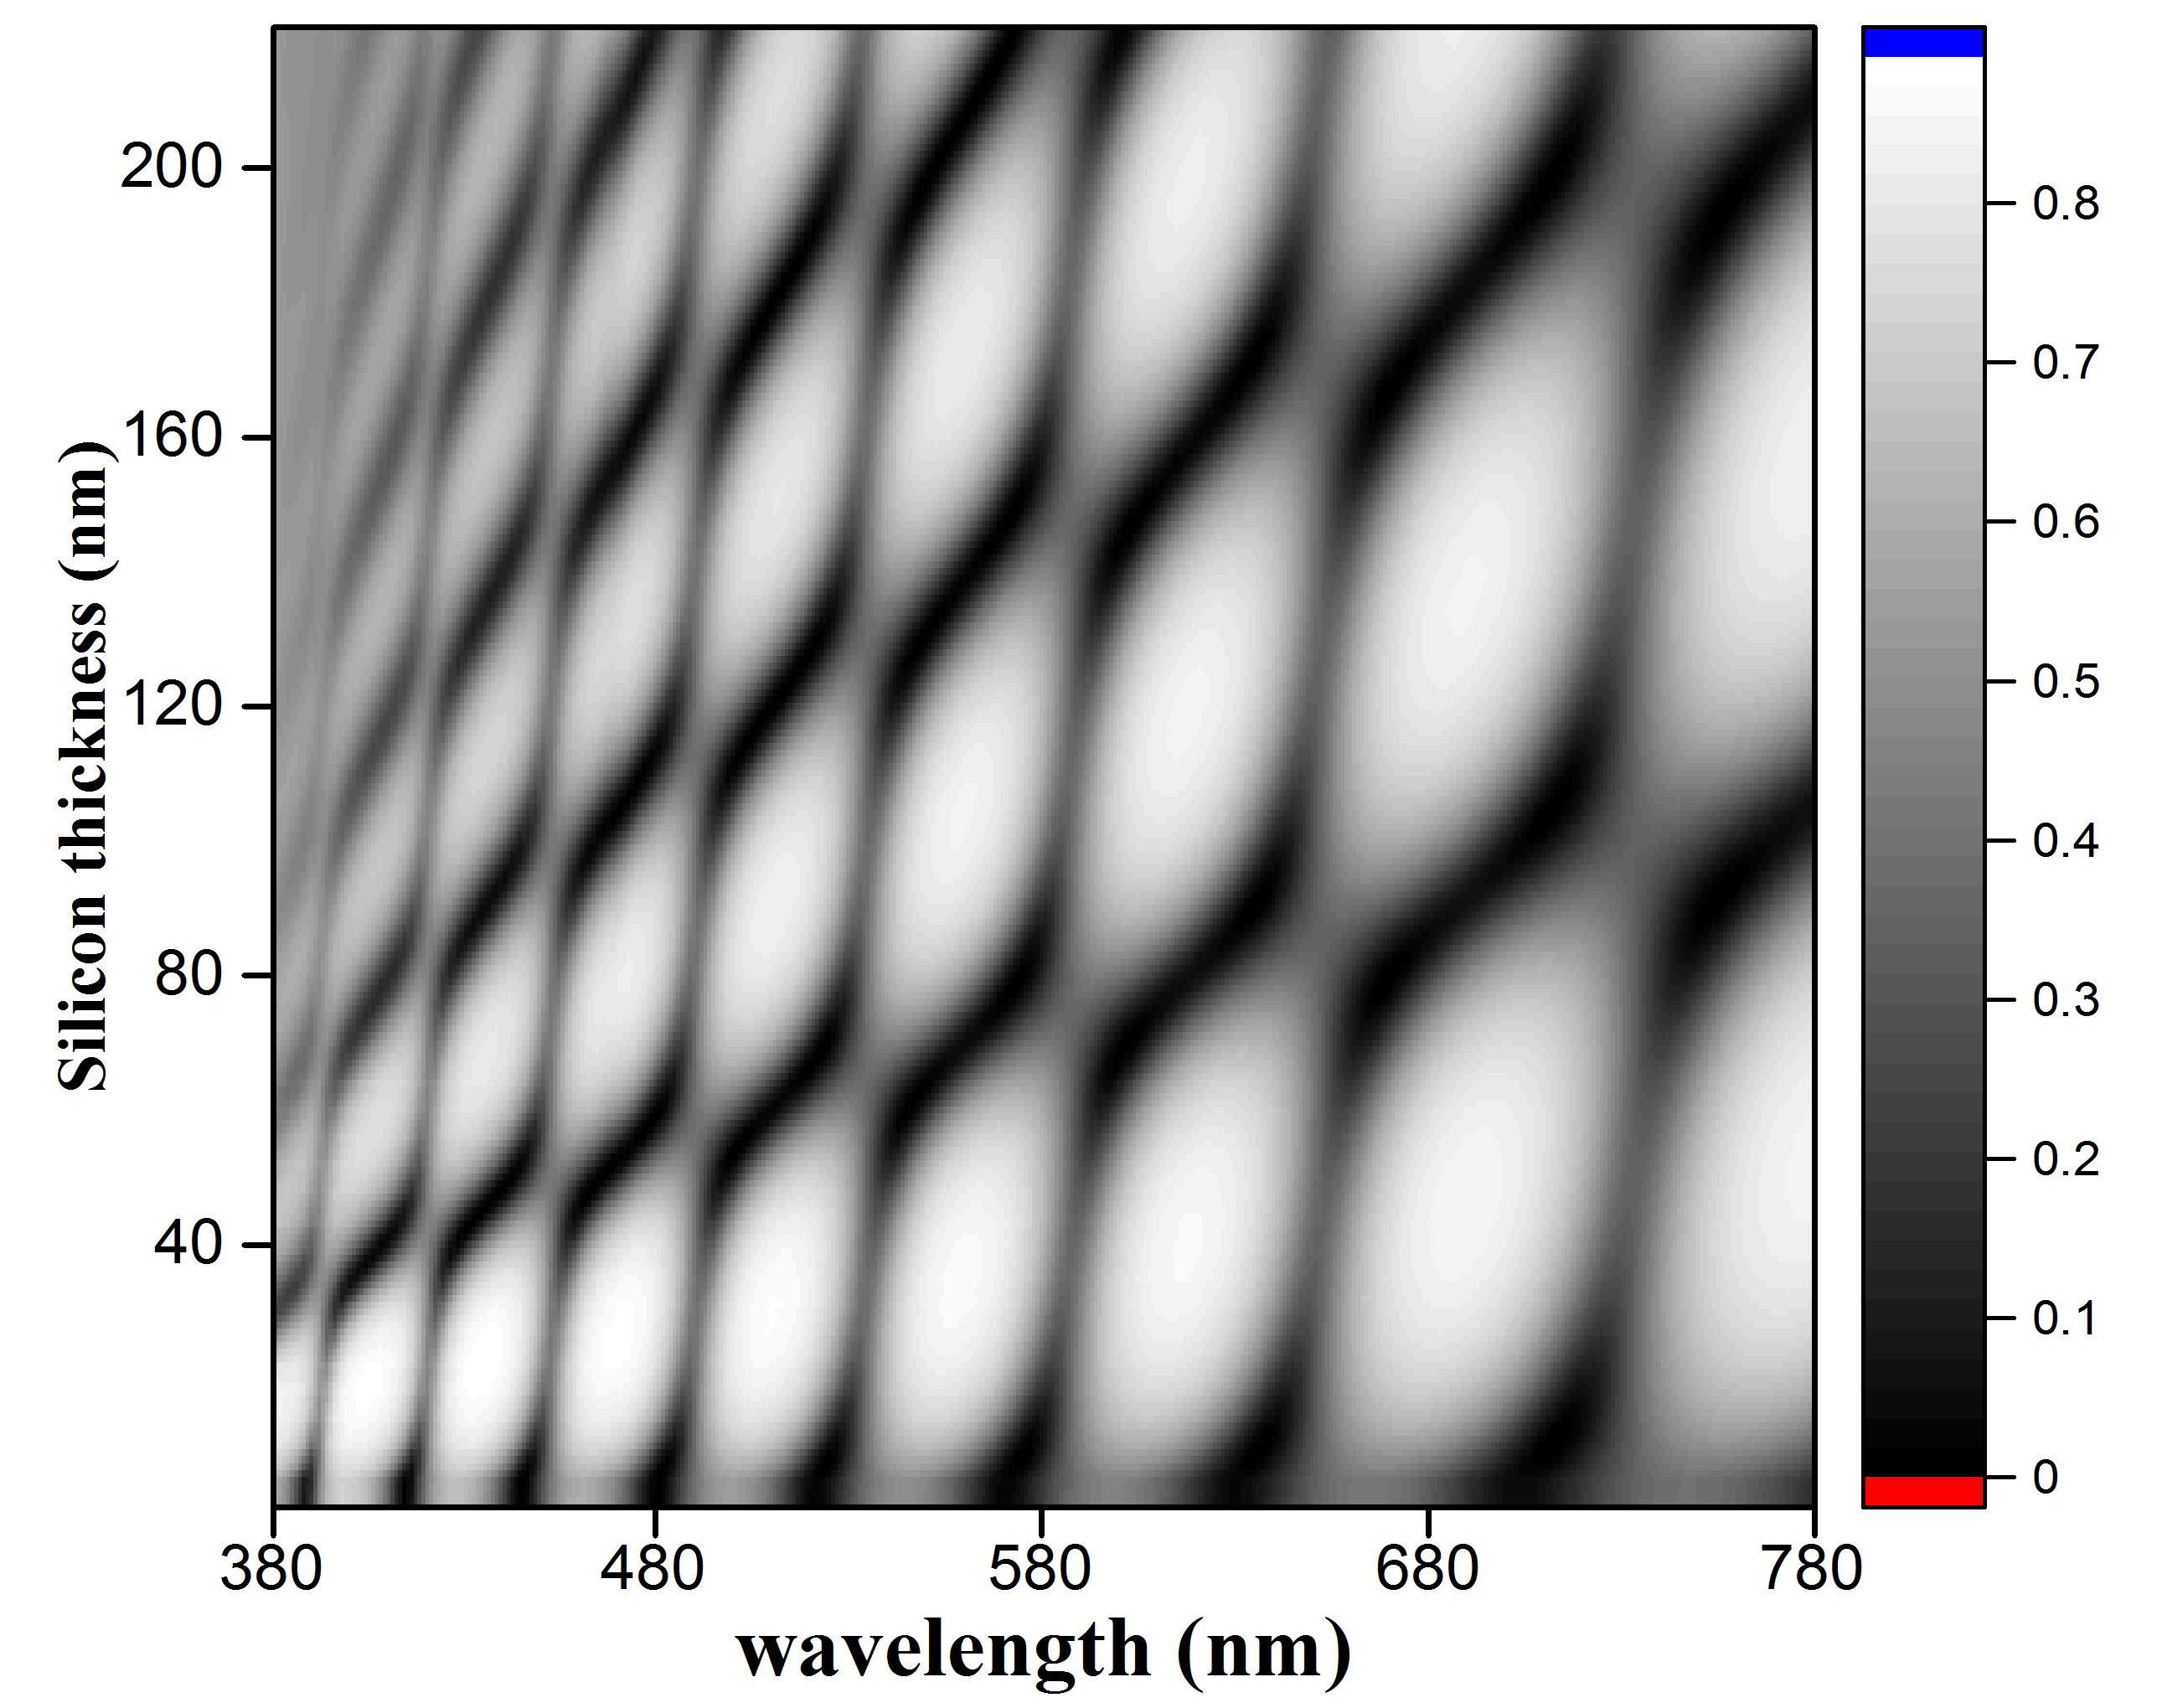
\includegraphics[width=12cm]{./Pictures/color_reflection_all.jpg}
	\captionsetup{justification=centering}
	\caption{FDTD solutions仿真得到不同硅层厚度下的反射谱}
	\label{color_reflection_all}
\end{figure}

得到了SOI芯片不同硅层厚度下的反射谱之后我们需要确定光源的光谱,因为对于SOI芯片来说它是不发光物体,根据上文所述,观察该类物体的光谱需要由光源和反射谱共同决定。假设在自然光下进行观察,采用日光光谱作为光源光谱,如图\ref{color_sun_spectrum}所示,我们只截取了太阳光谱中380~\~{}~780~$nm$这一段中的光谱,因为只有这一段与颜色有关,图中的光谱强度已经做了归一化处理。

\begin{figure}[htb]
	\centering
	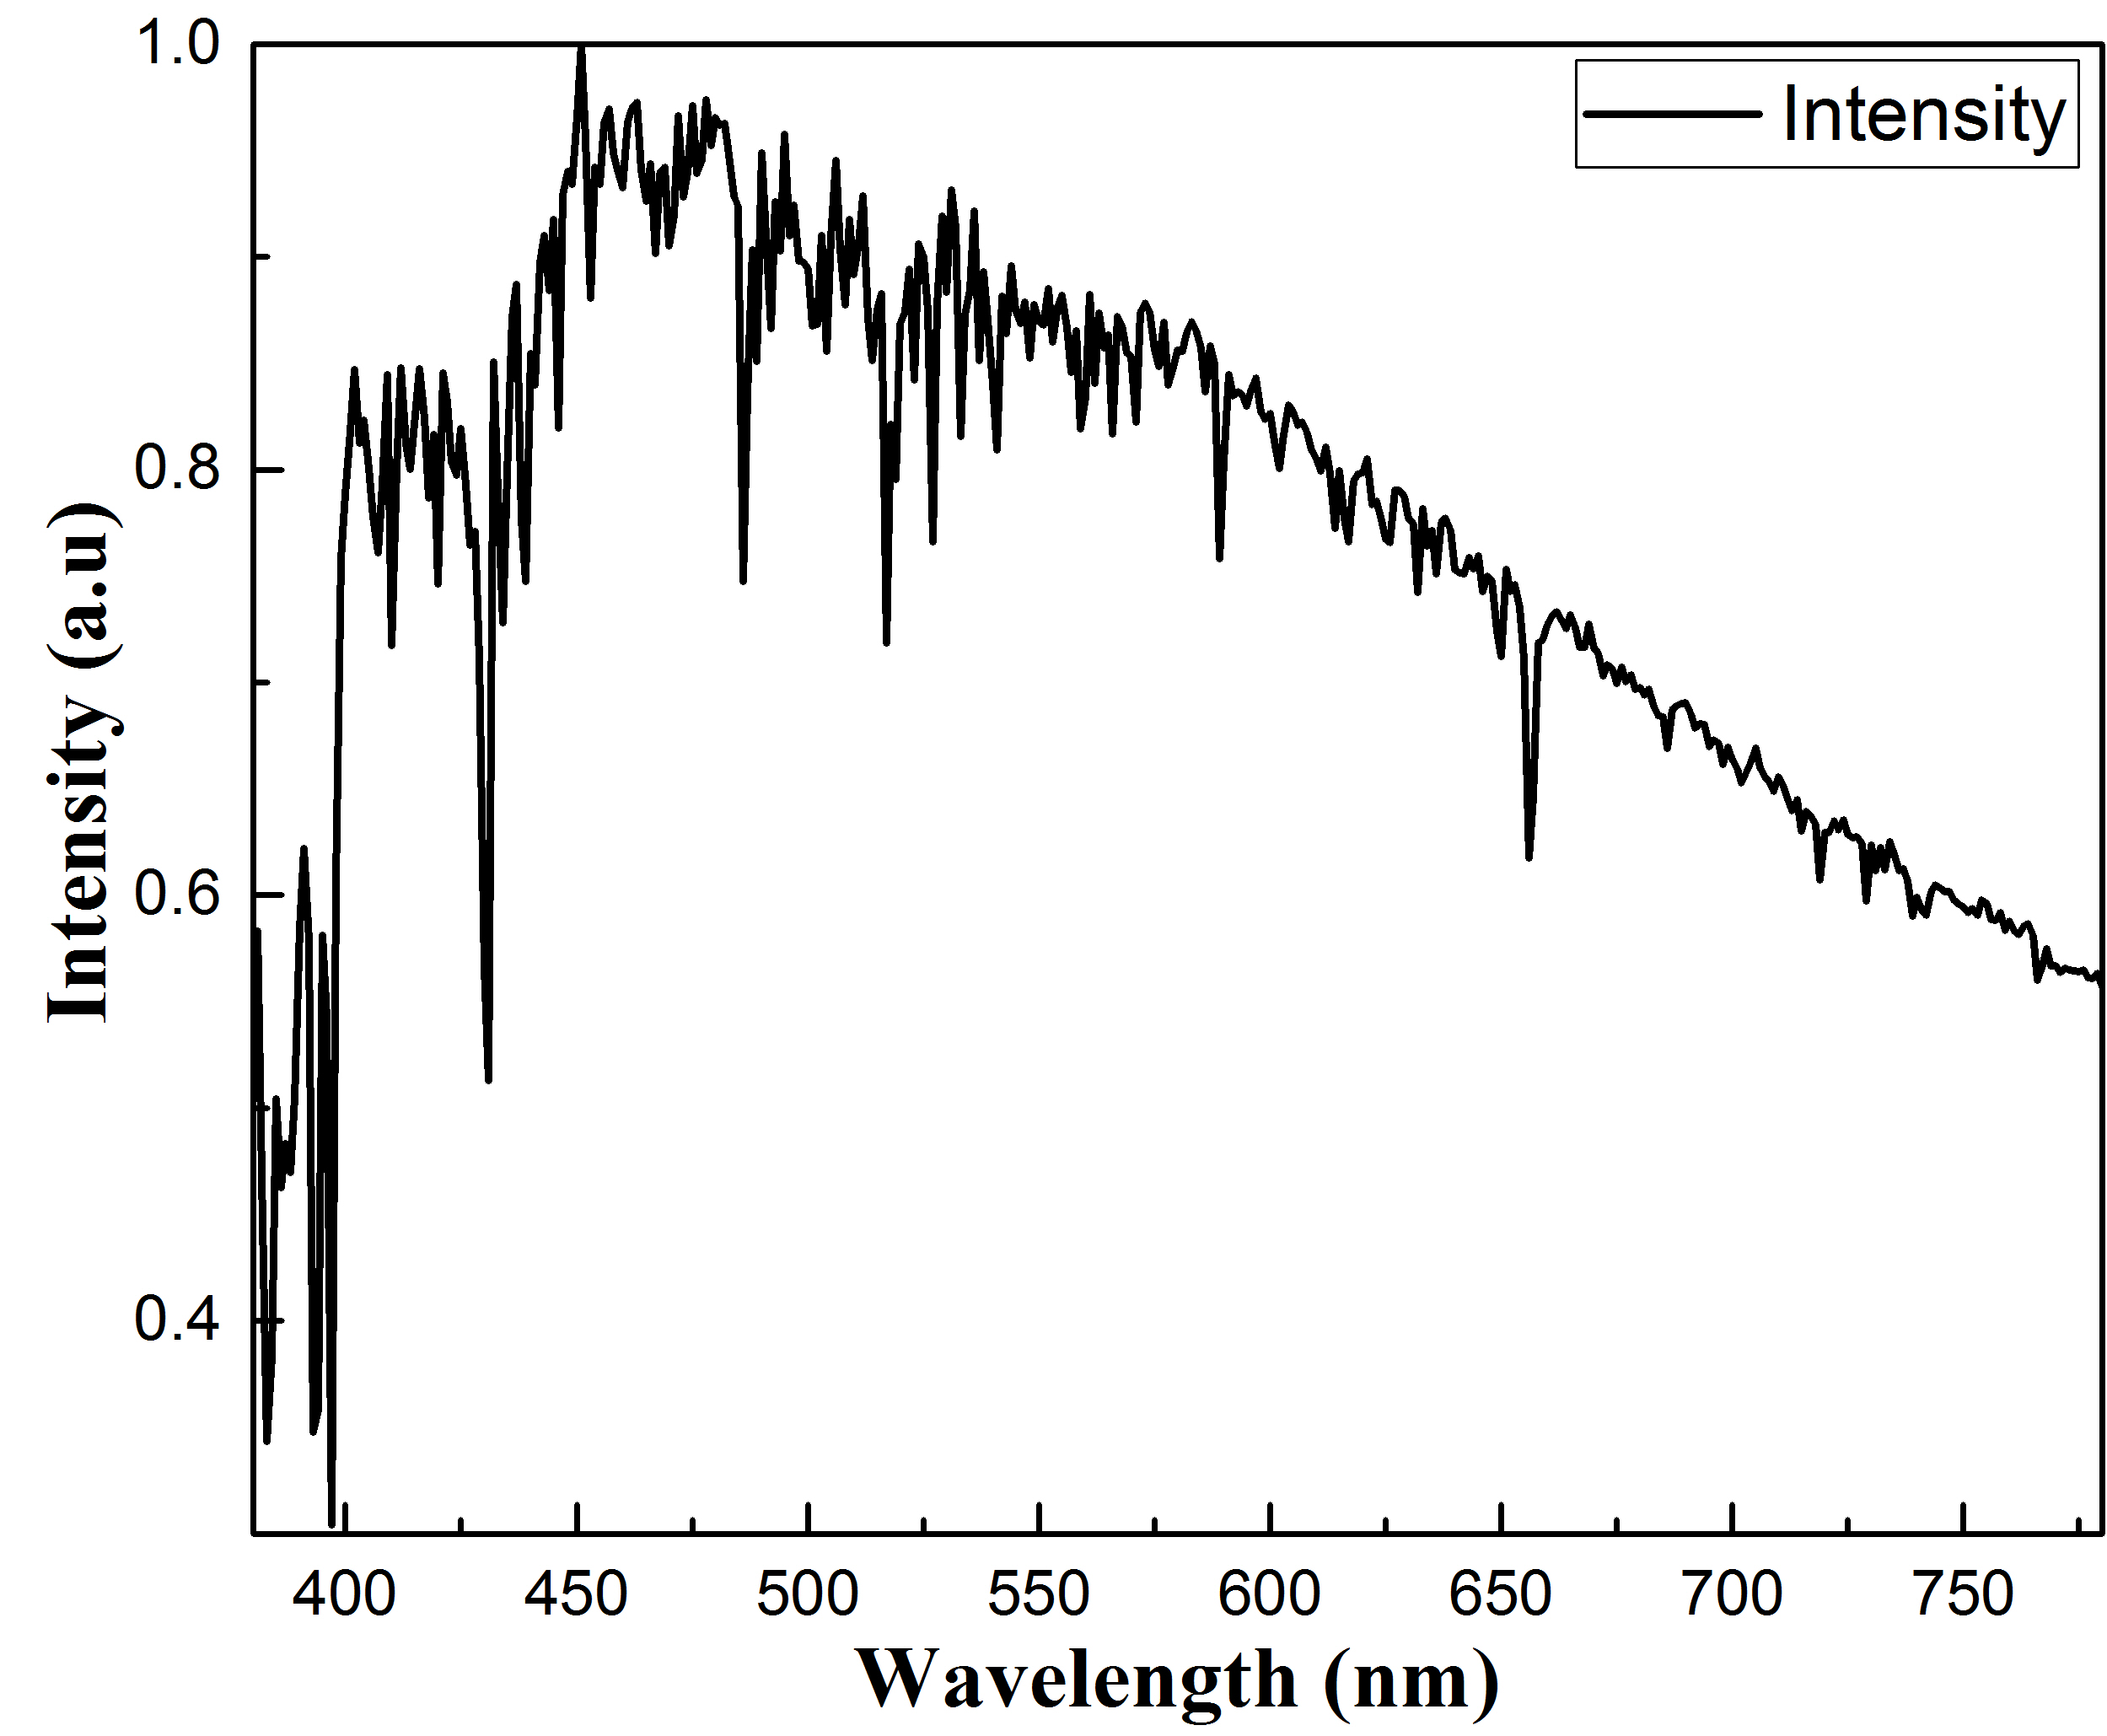
\includegraphics[width=12cm]{./Pictures/color_sun_spectrum.jpg}
	\captionsetup{justification=centering}
	\caption{380~nm~\~{}~780~nm波段的太阳光谱\cite{sunspectrum}}
	\label{color_sun_spectrum}
\end{figure}

将日光光谱与SOI芯片的反射谱相乘,得到最终用来计算色坐标的光谱之后,然后按上一节所述方法,计算得到不同硅层厚度对应的光谱的rgb坐标,显示之后的效果如图\ref{color_220nm}(a)所示,图中横坐标没有意义,只是重复了同一硅层厚度下的颜色以方便观察,纵坐标表示SOI芯片的硅层厚度。当硅层厚度为220~$nm$时,颜色显示为浅绿色,这与本章开头图\ref{color_wafer}(a)展示的硅层厚度为220~$nm$的标准SOI芯片的颜色是符合的。随着硅层厚度的减小,SOI芯片的颜色会先变成粉红,然后又变绿,再变粉红,之后会出现黄色,在硅层厚度在40~\~{}100~$nm$范围内时,颜色变化的信息非常丰富。这是由于硅的折射率实部很大,在可见光波段达到4以上,在波长为400~$nm$左右时,折射率甚至可以达到6左右,如图\ref{color_220nm}(b)所示,所以当硅层厚度减小时光程差变化比较大,干涉增强的波长值移动也会比较迅速。硅薄膜的颜色随厚度变化特性还跟硅对可见光的吸收相关,从图\ref{color_220nm}(c)中可以看到,硅对短波长的可见光比长波长的可见光吸收大,所以当硅薄膜厚度在100~$nm$以上时,短波长的可见光吸收较多,故颜色只有红、绿、黄色,缺少蓝色,当硅薄膜厚度减小到80~$nm$附近时,才有蓝色部分出现。当计算二氧化硅薄膜厚度变化的时候,颜色变化就会比硅缓慢很多且厚度较厚时也可以观察到蓝色。当硅层厚度小于40~$nm$之后,SOI芯片就只会显示出灰度的变化,并且随着硅层厚度降低,灰度值也越来越高。这个因硅层厚度减小而颜色发生变化的情形与肥皂泡的破裂很类似,我们知道,当肥皂泡刚形成时,形成肥皂泡的水膜比较厚,当可见光照射时,总会有某些波长得到干涉增强,某些波长干涉相消,从而产生彩色,而且随着水膜因为蒸发厚度较小时,干涉增强的波长会不停地发生变化,故我们可以看到肥皂泡的颜色不停地发生变化。当水膜减薄到一定程度后,就无法形成可见光波段的干涉增强,此时就没有彩色,故当肥皂泡的彩色消失时,说明肥皂泡的厚度也减小到了一定程度,离破裂也就不远了。在这里,SOI芯片的硅层就像肥皂泡的水膜,当彩色快消失时,说明硅层厚度也所剩无几了。

\begin{figure}[htb]
	\centering
	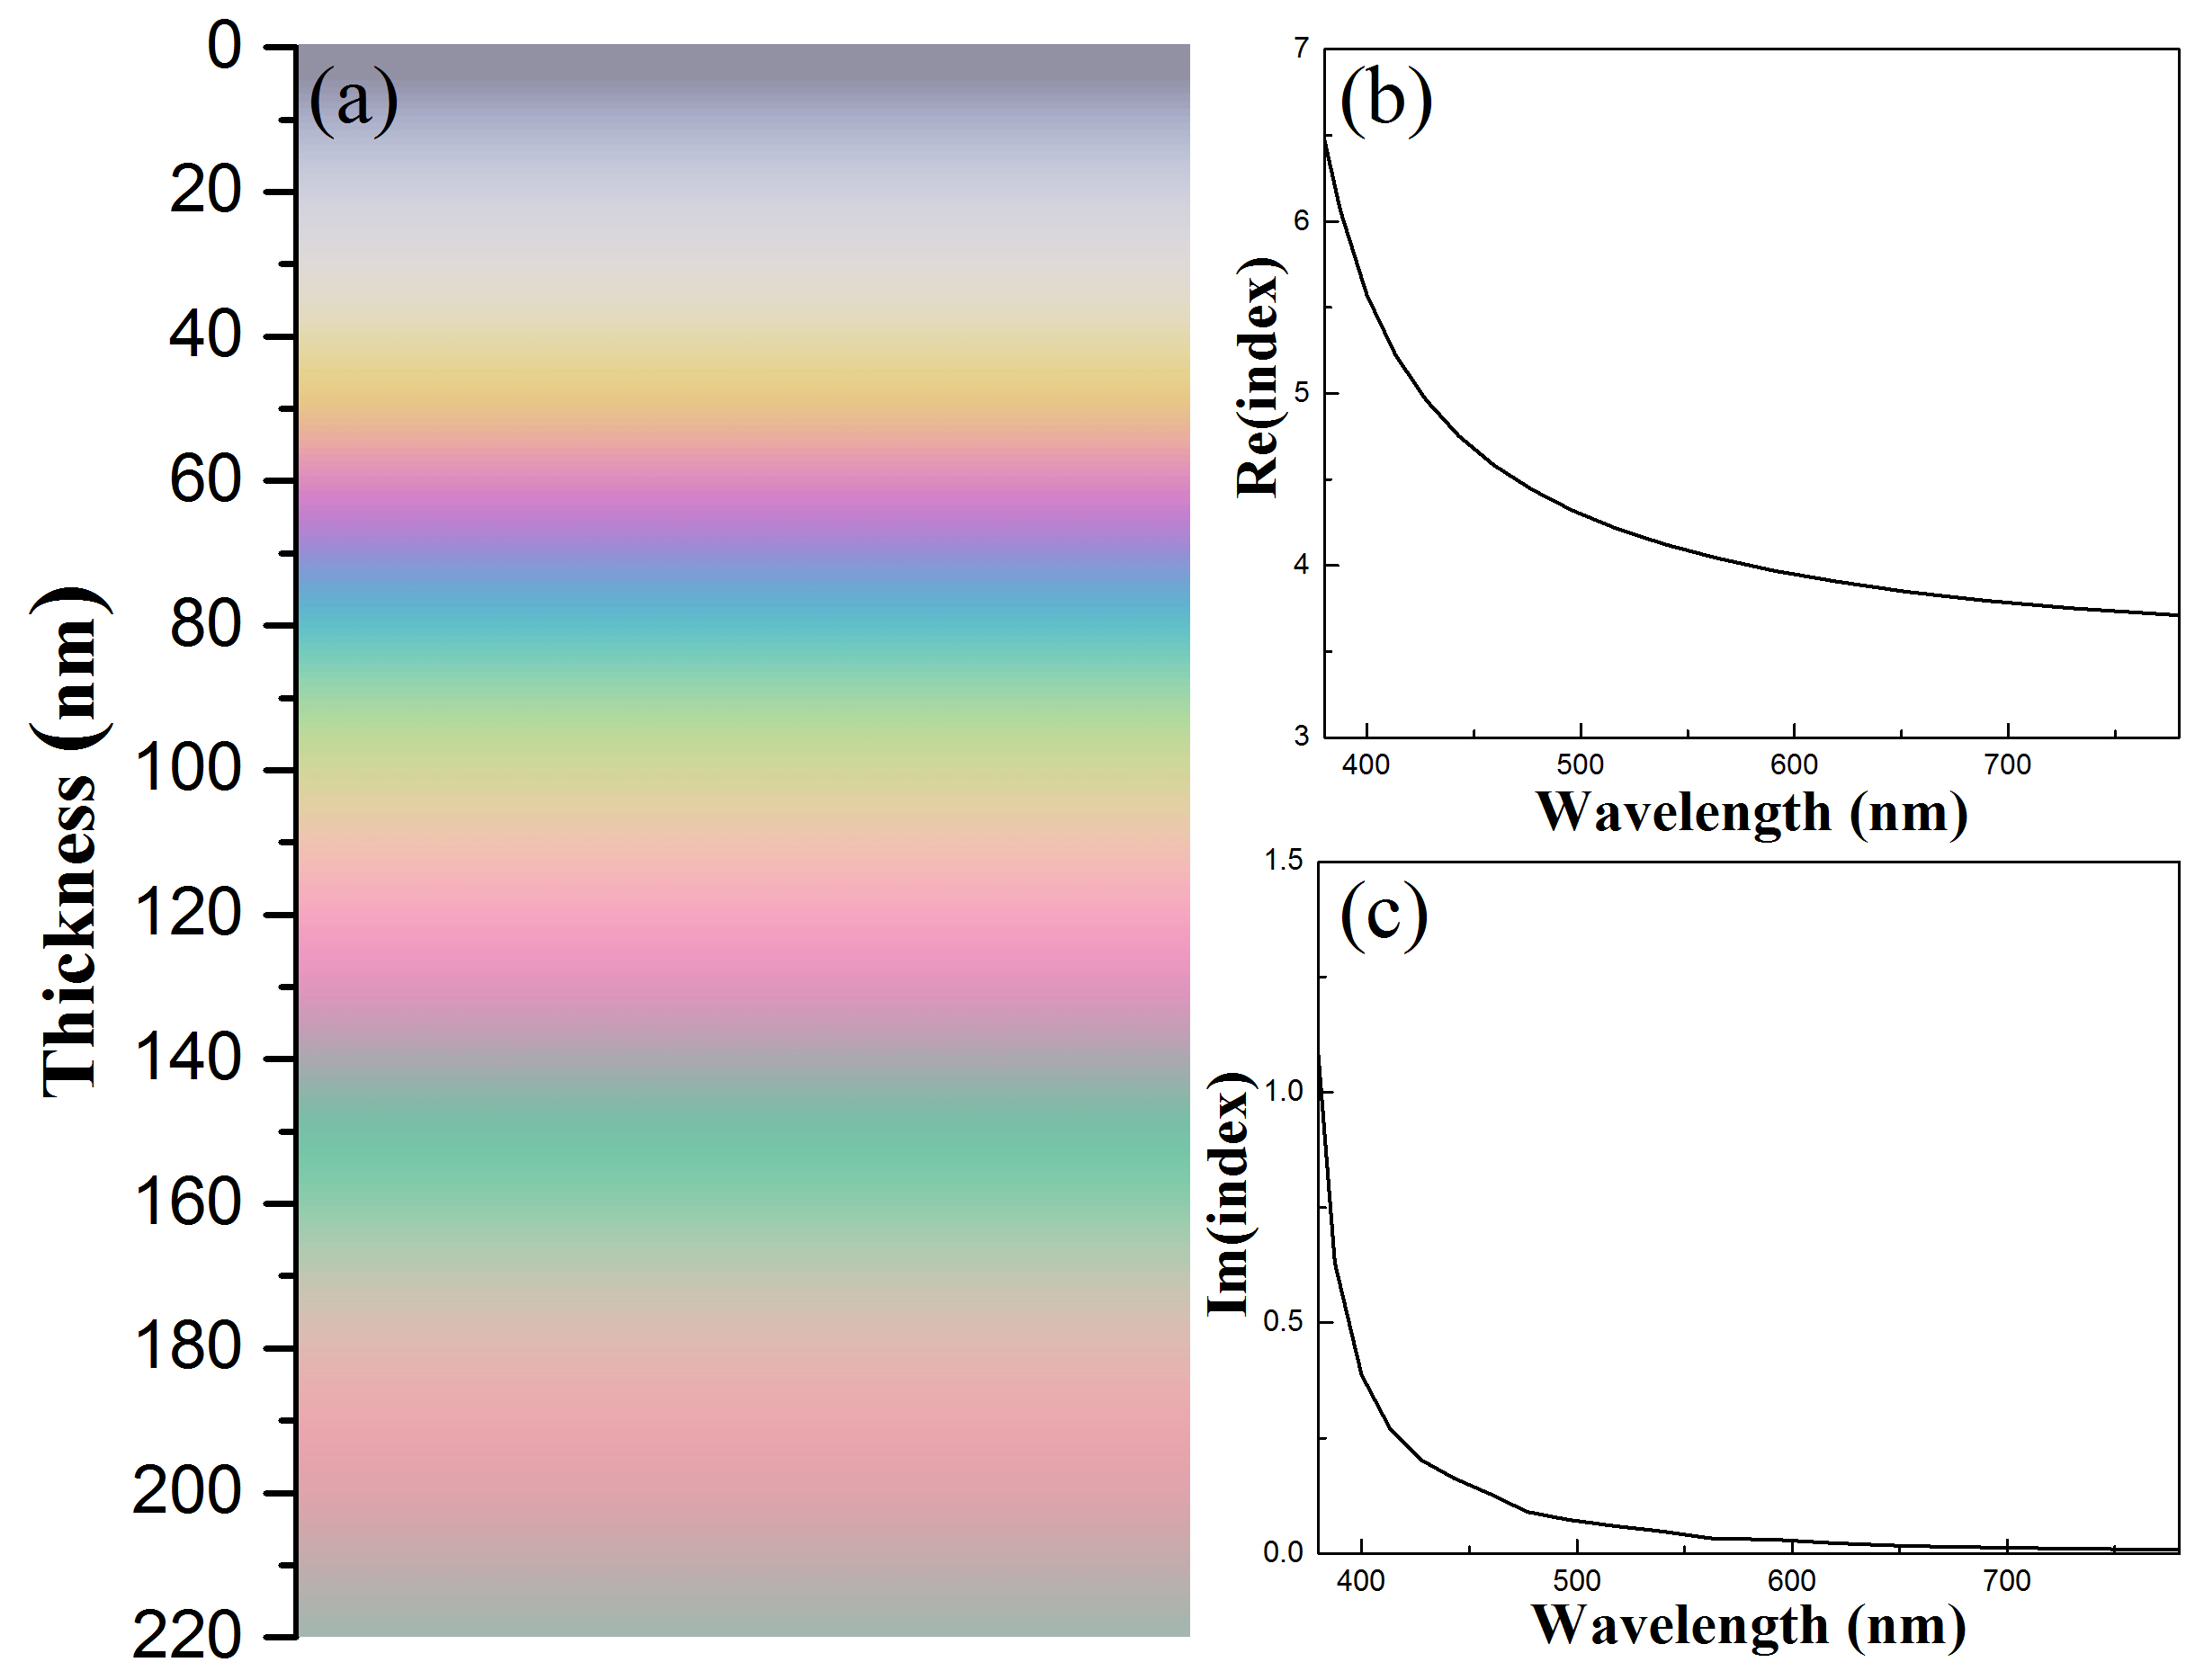
\includegraphics[width=14cm]{./Pictures/color_220nm.jpg}
	\captionsetup{justification=centering}
	\caption{(a)~0~\~{}~220~$nm$硅层厚度SOI芯片的色谱图;(b)硅在可见光波段的折射率实部;(c)硅在可见光波段的折射率虚部\cite{aspnes1983dielectric}}
	\label{color_220nm}
\end{figure}

为了比较不同角度入射光时观察到的颜色变化,我们计算了光源在30$^{\circ}$和60$^{\circ}$入射情况下SOI芯片随厚度变化的色谱图,如图\ref{color_compare}所示。我们可以看到当入射角度不同时,颜色变化很小,只是角度增大时,颜色明度值有所下降,这是由于入射角度增大时,反射率有所降低。根据计算结果,我们可以知道,当SOI芯片的硅层厚度确定之后,其颜色随观察角度的变化不明显,这个特性为我们接下来利用肉眼进行颜色比较确定硅层厚度提供了理论上的保证,因为SOI芯片表面光滑,往往会形成镜面反射从而使人脸成为背景色,影响颜色的判断。

\begin{figure}[htb]
	\centering
	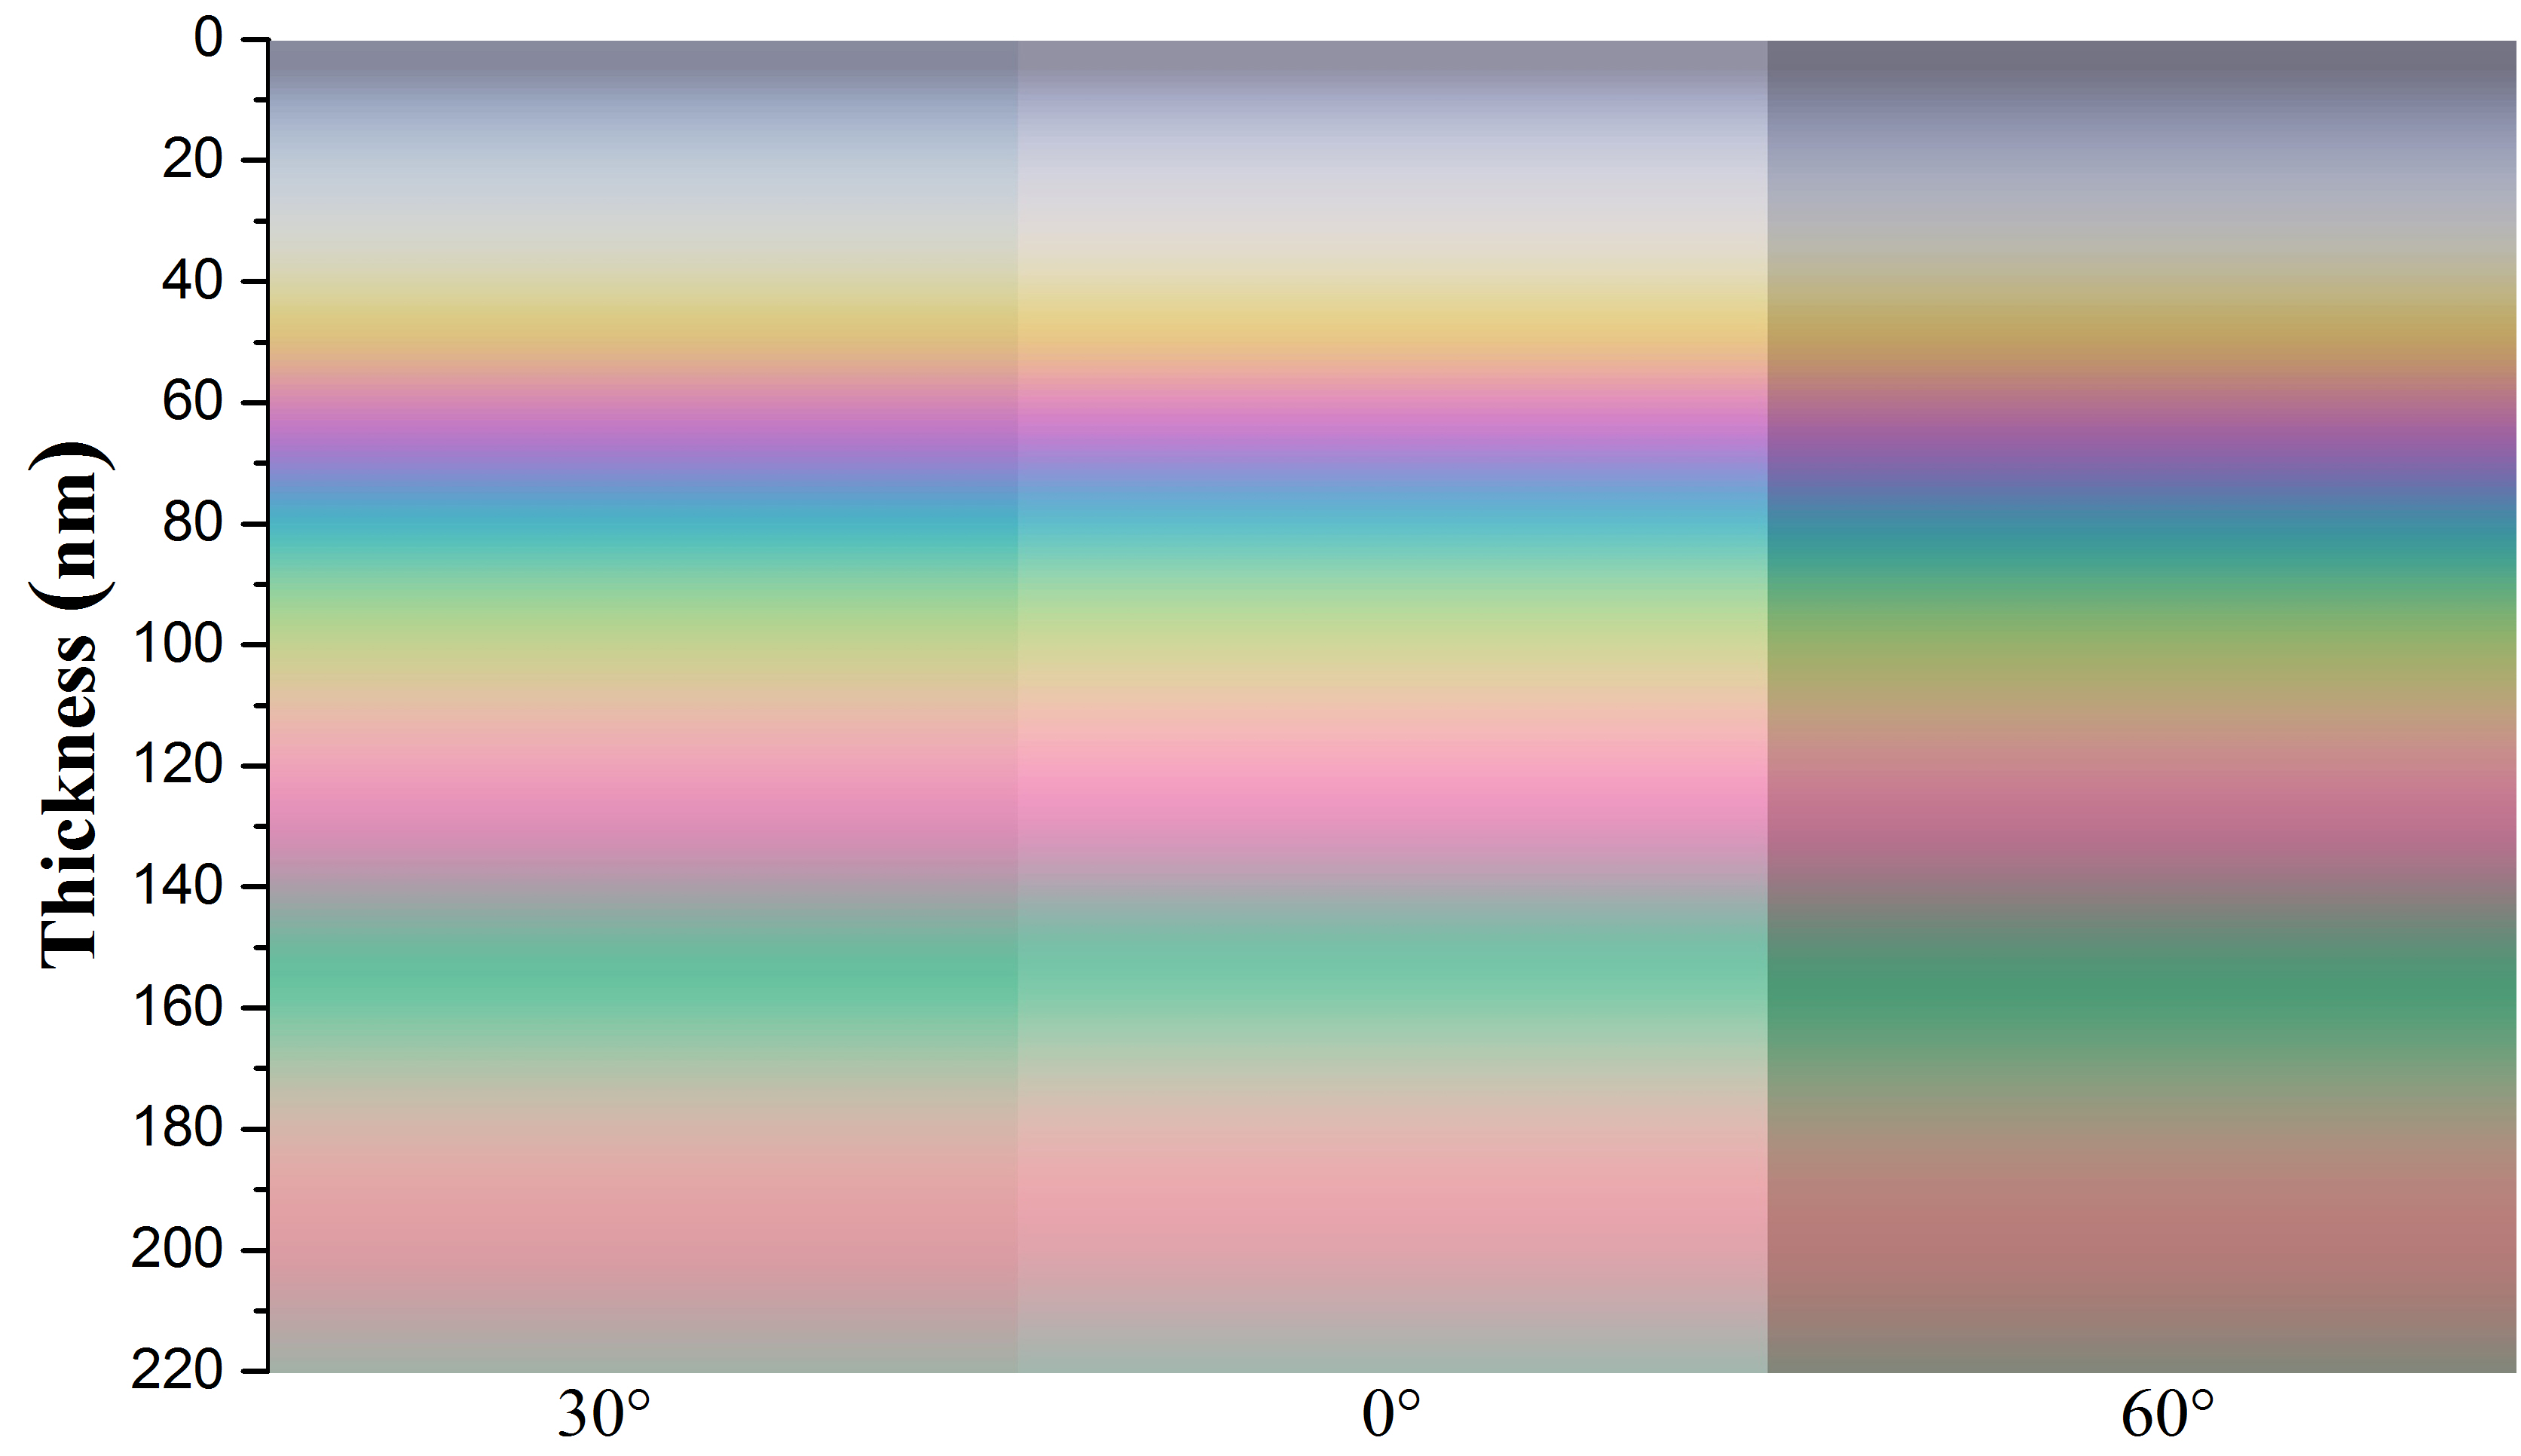
\includegraphics[width=14cm]{./Pictures/color_compare.jpg}
	\captionsetup{justification=centering}
	\caption{0$^{\circ}$、30$^{\circ}$、60$^{\circ}$观察时的色谱图}
	\label{color_compare}
\end{figure}

\section{颜色比较法测定硅层厚度}

为了方便颜色的比较,我们专门开发了一款叫做SOIEtch的手机APP,可以将色谱图中的颜色放大连续呈现,方便与芯片进行比较与匹配,软件截图如图\ref{color_app}所示。当上下滑动屏幕选取不同硅层厚度时,对应厚度的颜色会被放大呈现,选取与刻蚀之后的芯片颜色最相近的颜色,即可确定SOI芯片的硅层厚度。

\begin{figure}[htb]
	\centering
	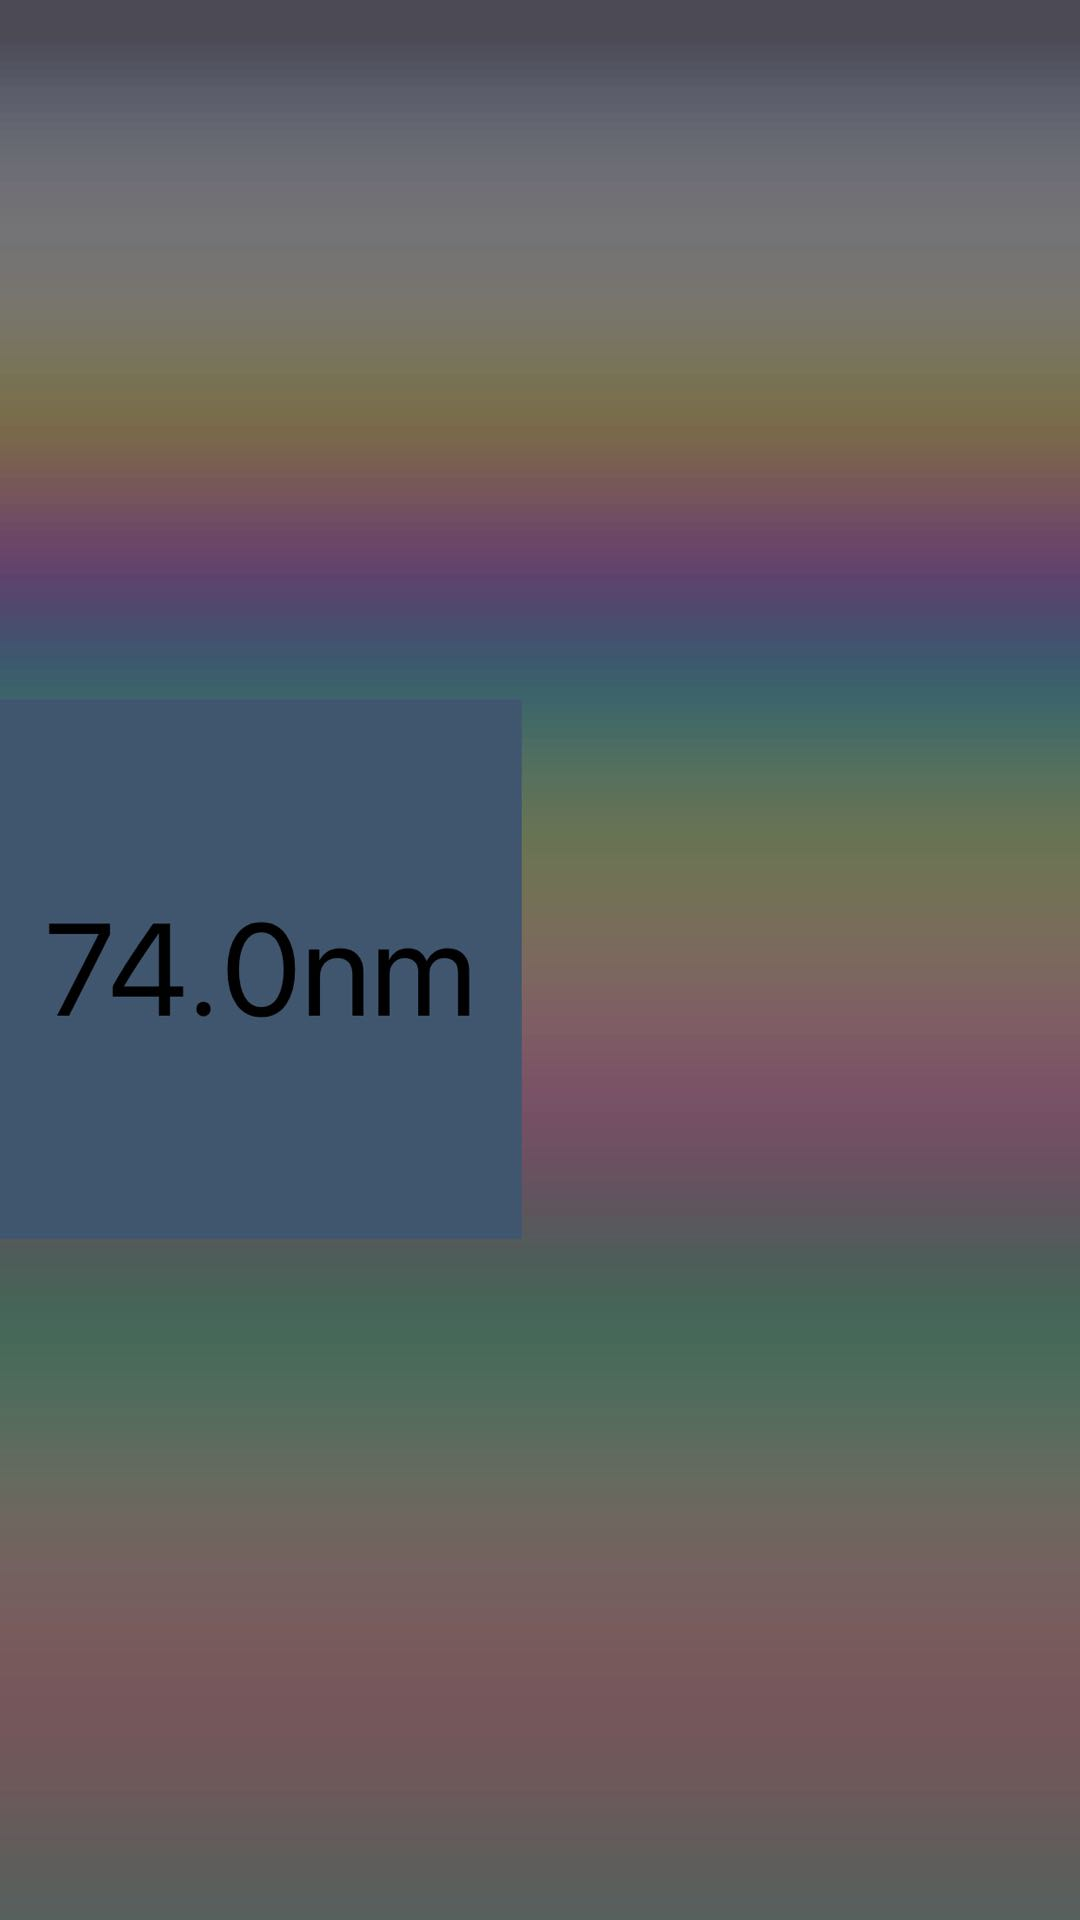
\includegraphics[width=6cm]{./Pictures/color_app.jpeg}
	\captionsetup{justification=centering}
	\caption{SOIEtch软件截图,插图为硅层厚度为74~$nm$时SOI芯片呈现的颜色}
	\label{color_app}
\end{figure}

我们制作了多组不同硅层厚度的SOI芯片,部分SOI芯片如图\ref{color_experiment}所示。根据SOIEtch软件测试,图\ref{color_experiment}(a)中心刻蚀深度155~$nm$,即中心剩余硅层厚度为65~$nm$。可以看到,ICP刻蚀时边缘刻蚀速率比较快,所以最边缘已经显示灰色,中间过渡区域是黄色,与计算结果相一致。图\ref{color_experiment}(b)中心刻蚀深度125~$nm$,即中心剩余硅层厚度为95~$nm$。可以看到,此时ICP刻蚀时还是边缘刻蚀速率比较快,但刻蚀速率分布与图\ref{color_experiment}(a)并不相同,这是由于两次刻蚀时底部的导热胶分布状况不同所致。

\begin{figure}[htb]
	\centering
	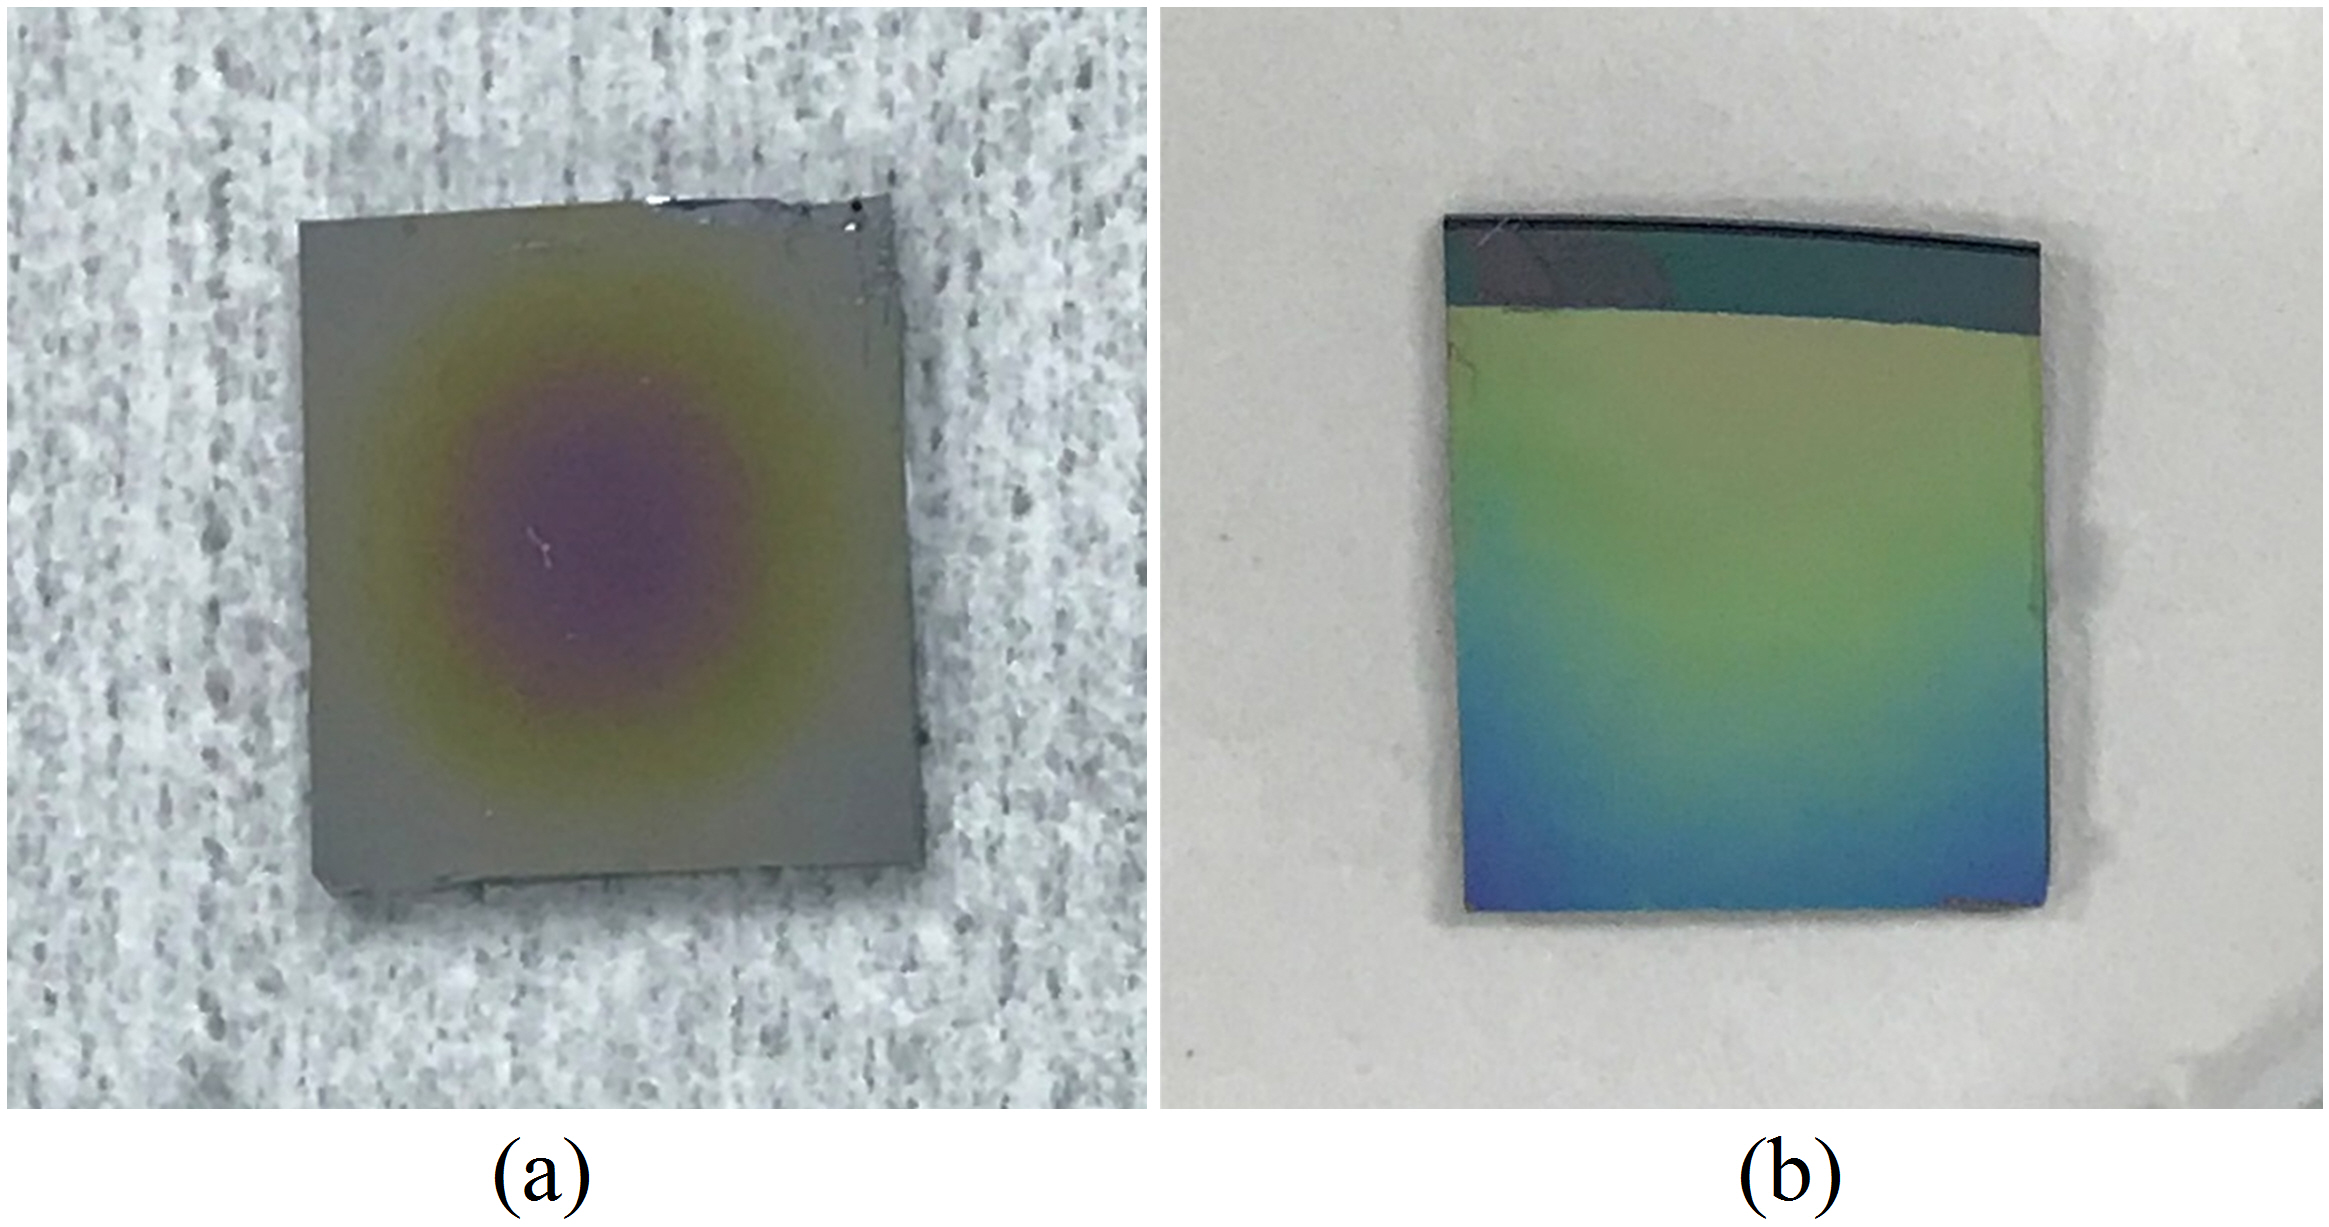
\includegraphics[width=12cm]{./Pictures/color_experiment.jpg}
	\captionsetup{justification=centering}
	\caption{ICP刻蚀之后的SOI芯片,(a)中心硅层厚度65~$nm$;(b)中心硅层厚度90~$nm$}
	\label{color_experiment}
\end{figure}

为了验证该方法的可靠性,我们利用SEM对SOI芯片的硅层厚度进行了测量作为标准值,然后让7名实验者利用SOIEtch软件,通过颜色比较法,读取对应SOI芯片的厚度,与标准值进行比较,所得结果如图\ref{color_experiment_measure}所示。从图中可以看到,当硅层厚度较大时,由于颜色变化比较缓慢,实验者利用颜色比较法测得的硅层厚度误差较大,且标准差也较大,这是由于颜色比较法是一种比较主观的方法,每个人对颜色相同的判断会有一定的差别,尤其是当颜色随厚度变化比较缓慢时;当硅层厚度较小时,由于颜色变化比较快速,实验者利用颜色比较法测得的硅层厚度误差较小,且标准差也较小。根据实验结果可以得知,当SOI芯片的硅层厚度小于120~$nm$时,利用颜色比较法测得的硅层厚度平均值与SEM测得的厚度值误差最大值为5.66~$nm$,考虑到SEM测得的硅层厚度也存在一定误差,有理由相信,该方法的实际误差将比5.66~$nm$更小。而且从图中还可以看到,当硅层厚度范围在40~\~{}80~$nm$时,通过颜色比较法测得的硅层厚度与SEM测得的厚度误差不超过2~$nm$,这已经足够满足大部分使用场景的需求。

\begin{figure}[htb]
	\centering
	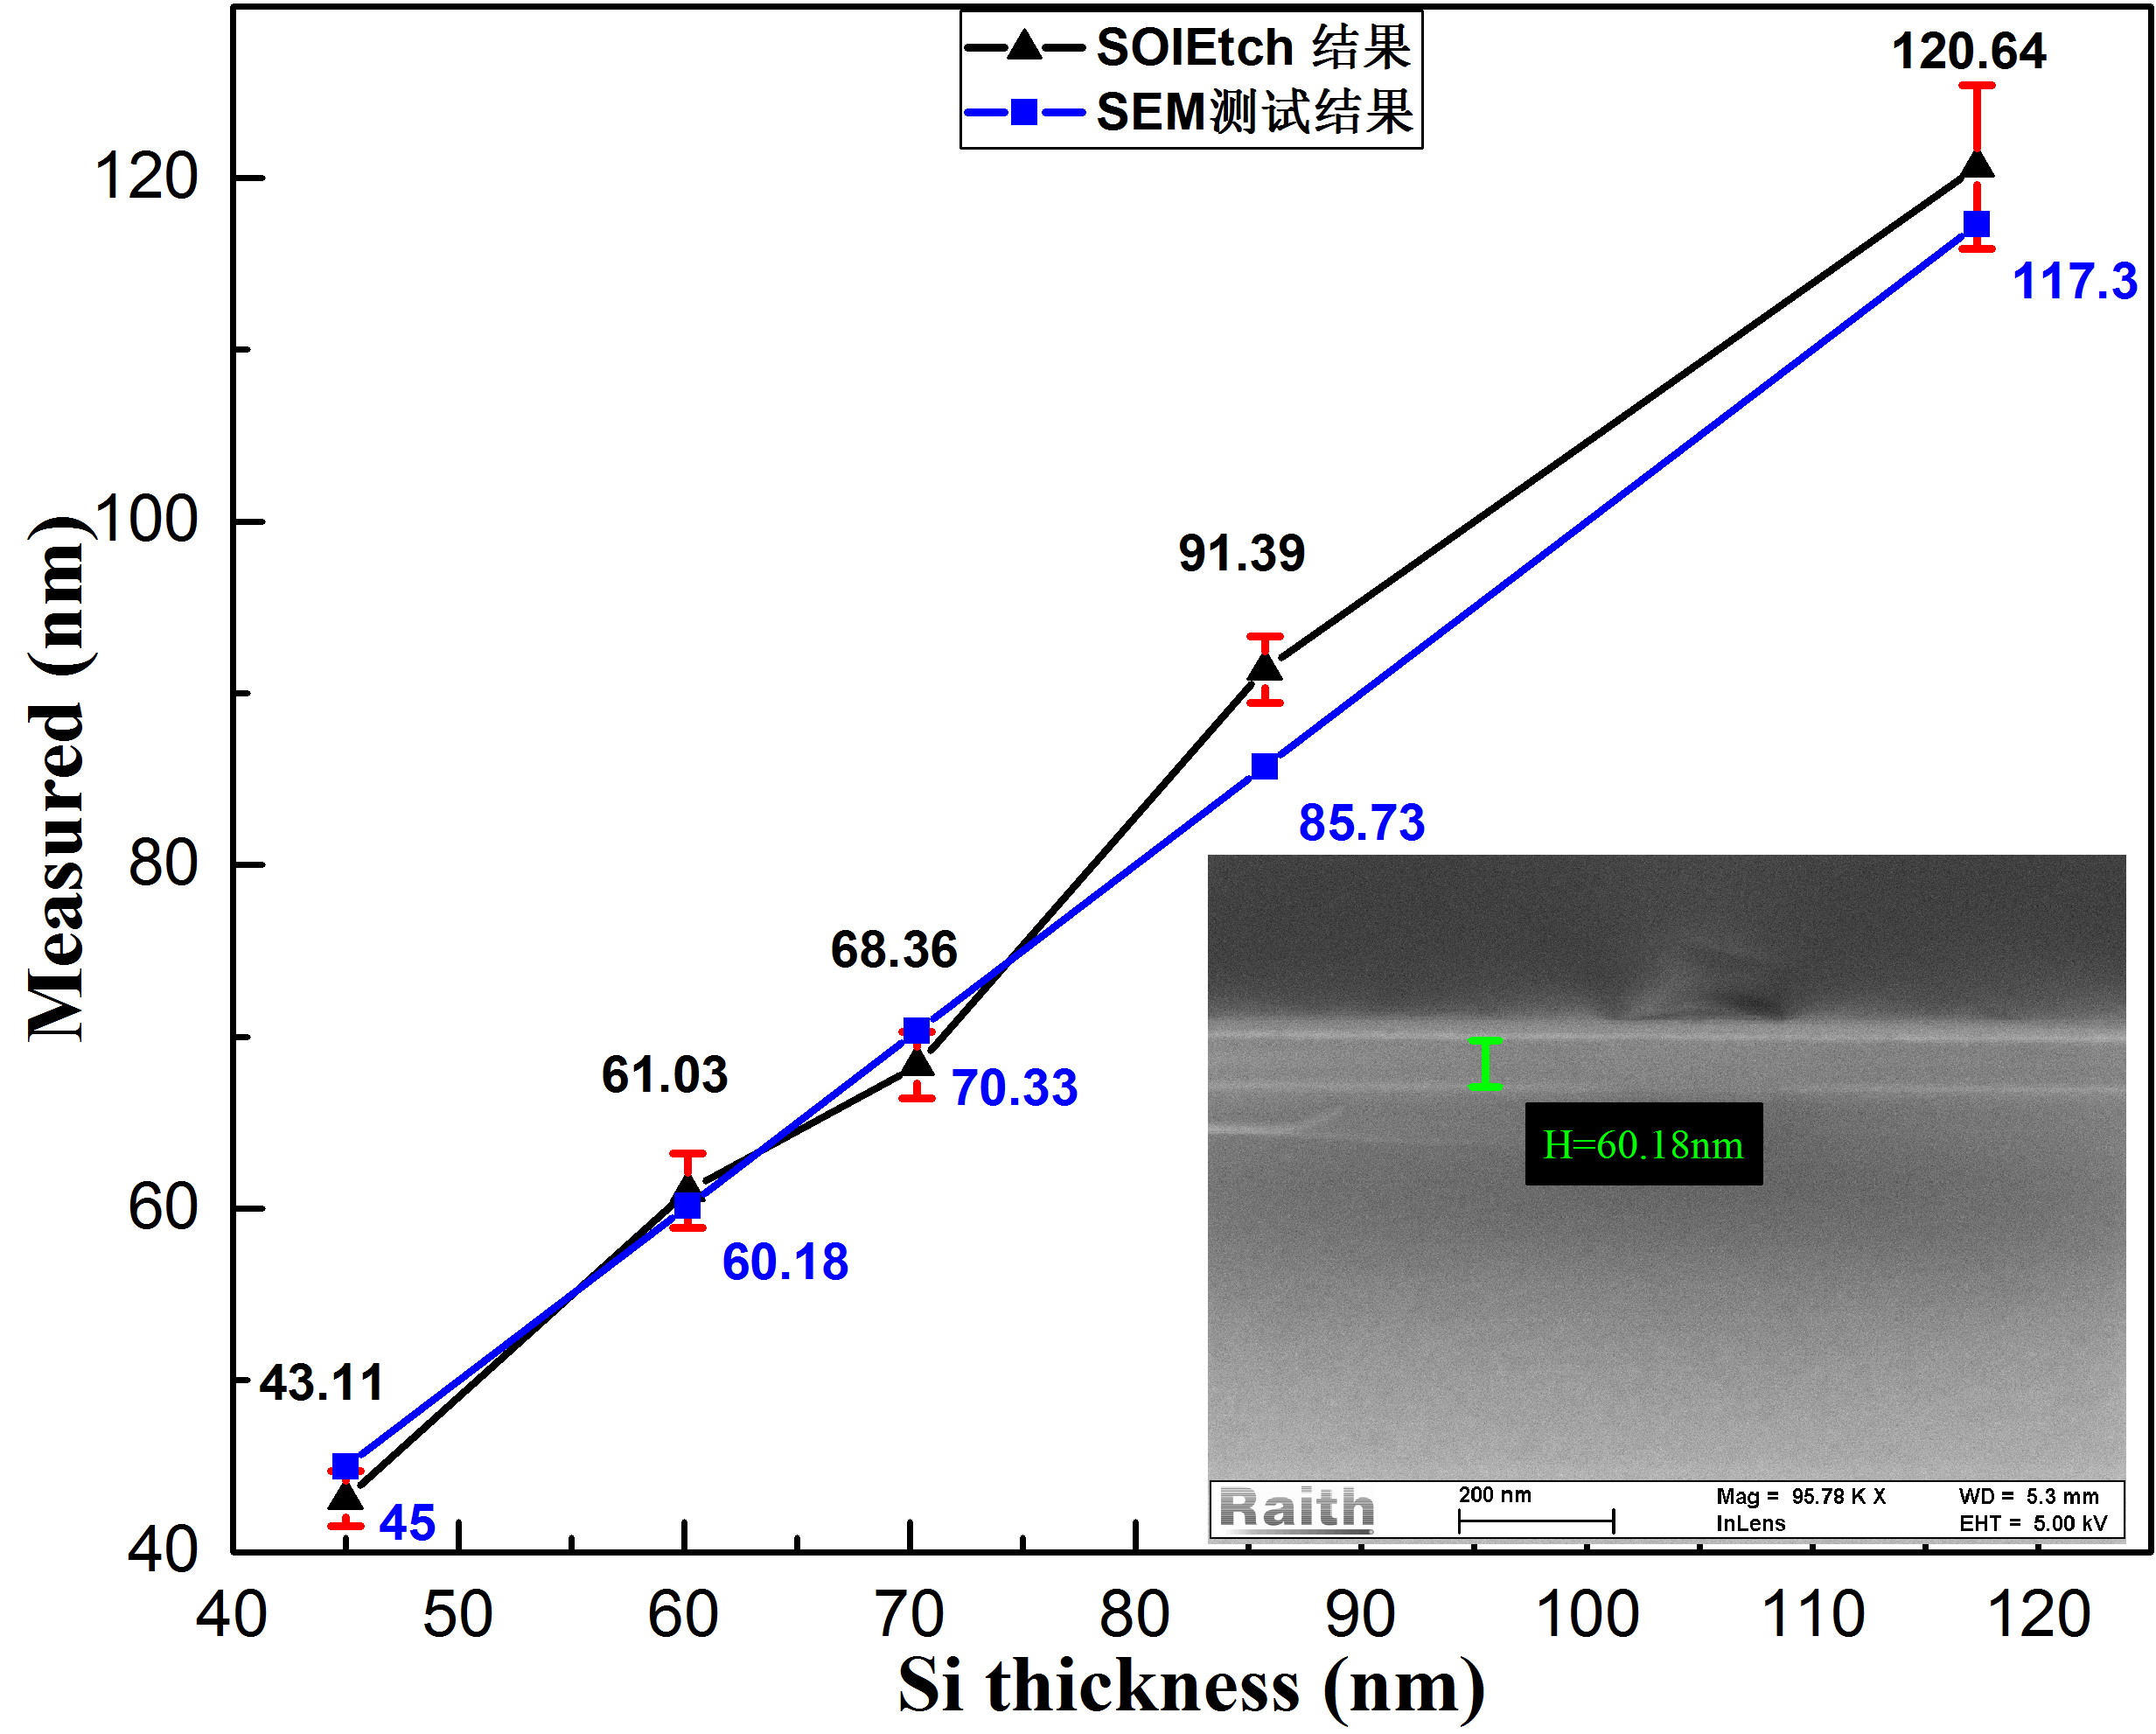
\includegraphics[width=13cm]{./Pictures/color_experiment_measure.jpg}
	\captionsetup{justification=centering}
	\caption{SEM与颜色比较法测得的硅层厚度比较,插图为SEM测试图}
	\label{color_experiment_measure}
\end{figure}

考虑到有的SOI芯片硅层较厚,我们用同样的方法计算了SOI芯片硅层厚度为0~\~{}~400~$nm$时的色谱图,如图\ref{color_400nm}所示。我们可以看到随着SOI芯片的硅层厚度越来越大,颜色的饱和度也越来越低,色调也只在红色和绿色之间转换,再利用颜色比较法来测定硅层厚度误差也将变大,此时该方法就不再适用。

\begin{figure}[htb]
	\centering
	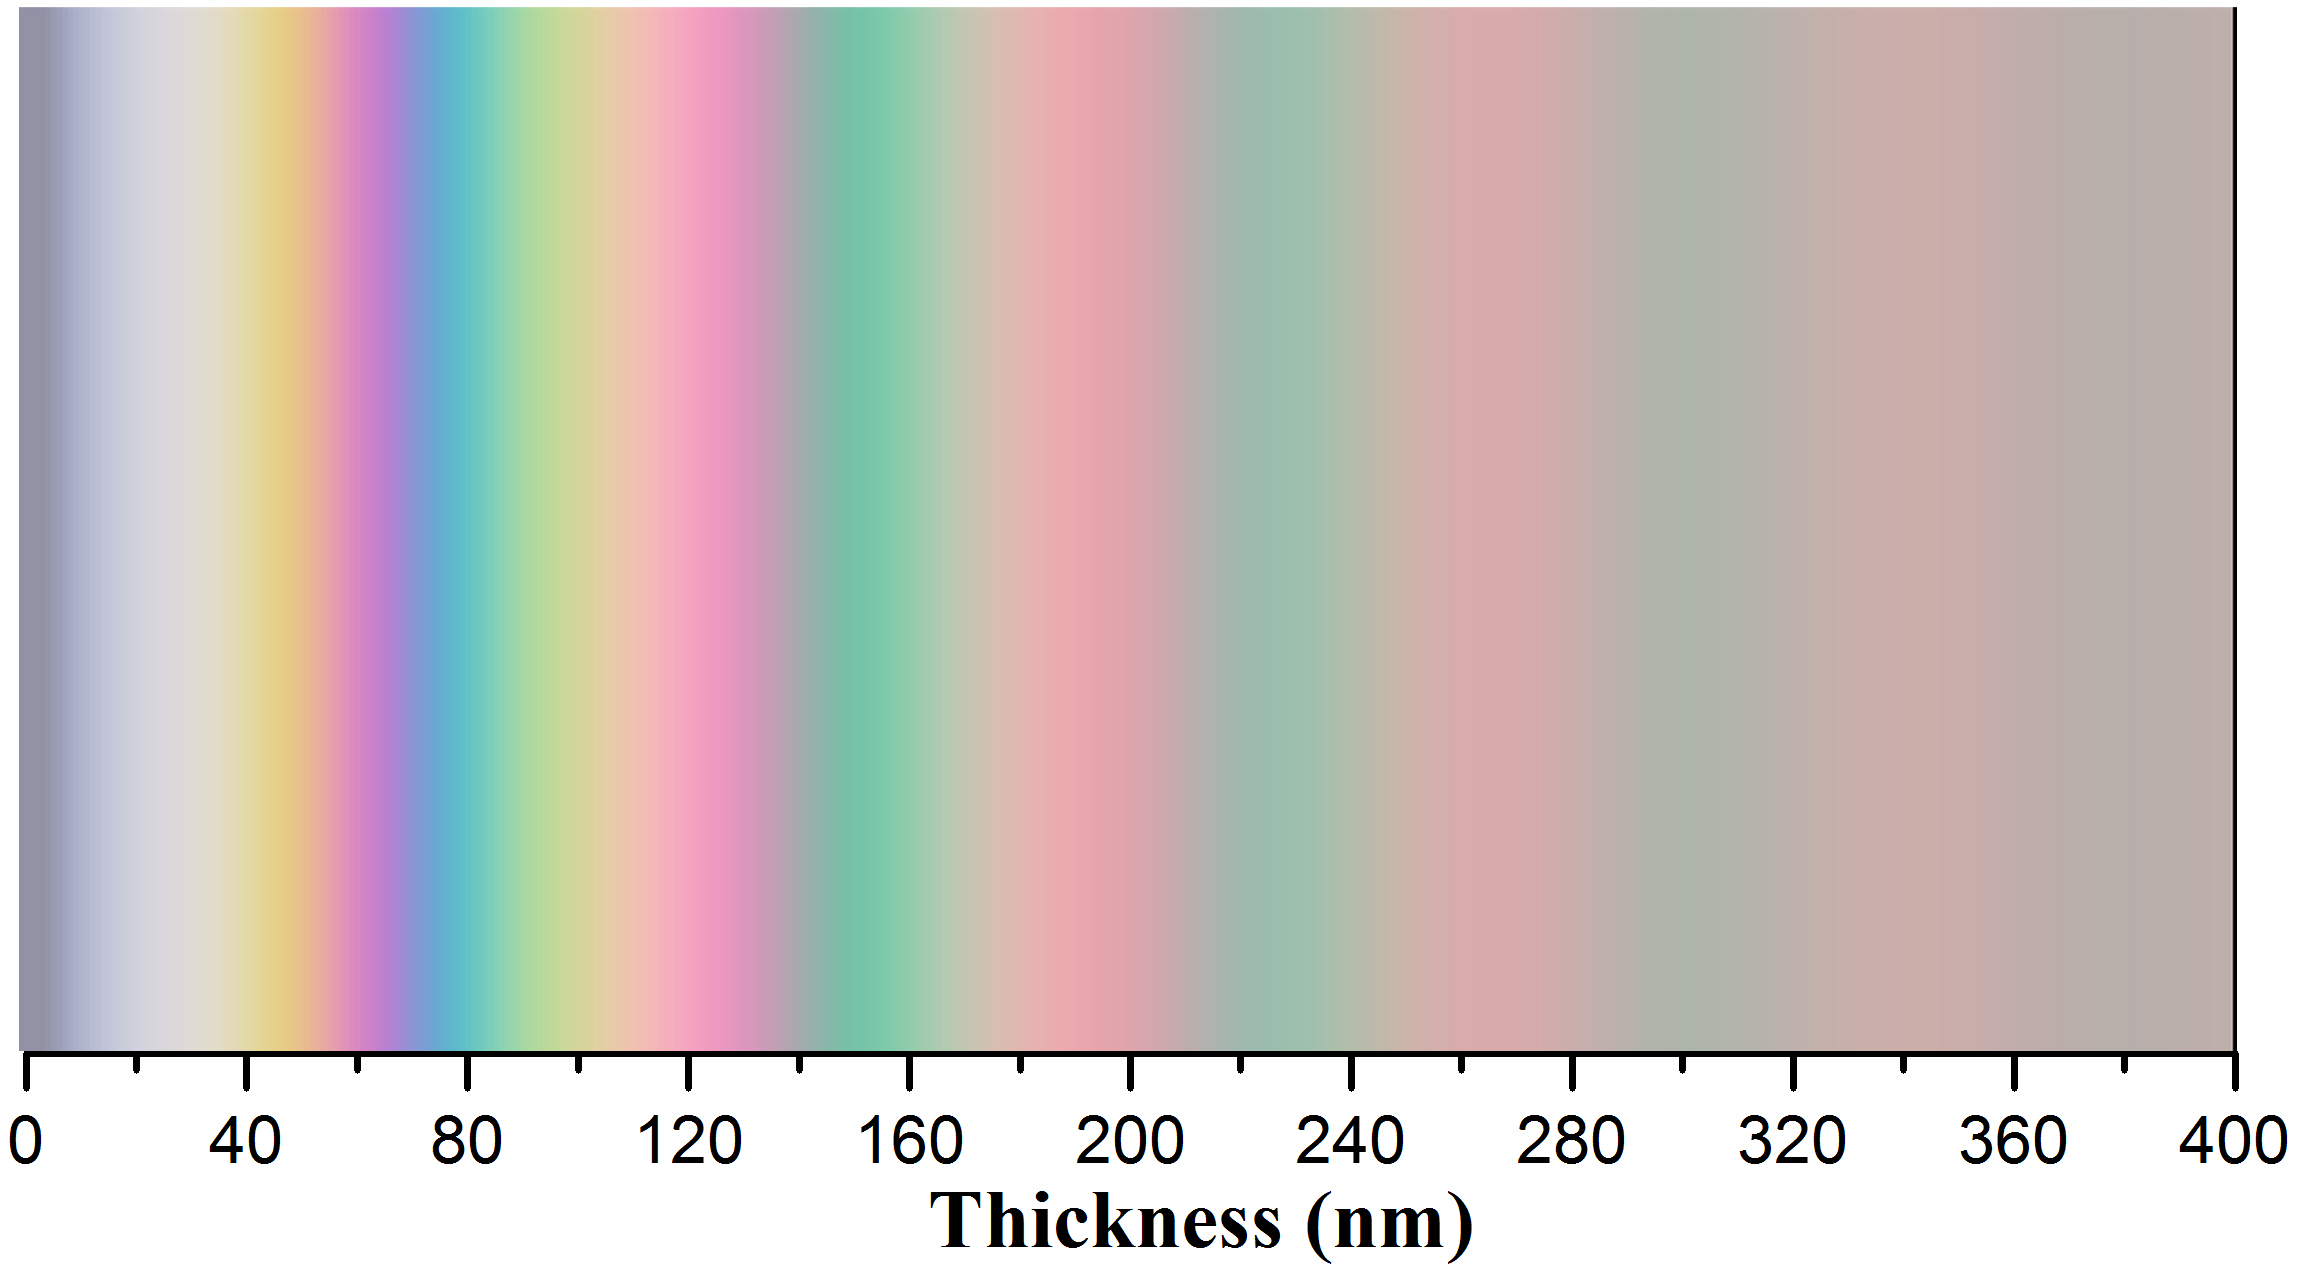
\includegraphics[width=13cm]{./Pictures/color_400nm.jpg}
	\captionsetup{justification=centering}
	\caption{0~\~{}~400~$nm$硅层厚度SOI芯片的色谱图}
	\label{color_400nm}
\end{figure}

\section{本章小结}

本章首先介绍了薄硅器件利用其低损耗等特性在集成器件领域的应用,以及目前获得薄硅的两种方法,ICP刻蚀法和热氧法。这两种方法都需要通过减薄现有SOI芯片的硅层厚度来实现,基于此本文提出了一种利用颜色比较法来帮助快速判断SOI芯片硅层厚度的方法。之后介绍了一些光度学与色度学的基础知识作为该颜色比较法的理论基础,然后通过数值仿真的方法计算得到SOI芯片不同硅层厚度的色谱图,给出了SOI芯片显示的颜色与硅层厚度之间的关系,并从理论上进行了分析。最后,专门开发了一款手机APP SOIEtch用来辅助颜色判断。经过实验测试,当硅层厚度小于120~$nm$时,颜色比较法测得的结果与SEM测得的结果相比较,可以达到较高的精度。







